\documentclass{book}
\usepackage[a4paper,top=2.5cm,bottom=2.5cm,left=2.5cm,right=2.5cm]{geometry}
\usepackage{makeidx}
\usepackage{natbib}
\usepackage{graphicx}
\usepackage{multicol}
\usepackage{float}
\usepackage{listings}
\usepackage{color}
\usepackage{ifthen}
\usepackage[table]{xcolor}
\usepackage{textcomp}
\usepackage{alltt}
\usepackage{ifpdf}
\ifpdf
\usepackage[pdftex,
            pagebackref=true,
            colorlinks=true,
            linkcolor=blue,
            unicode
           ]{hyperref}
\else
\usepackage[ps2pdf,
            pagebackref=true,
            colorlinks=true,
            linkcolor=blue,
            unicode
           ]{hyperref}
\usepackage{pspicture}
\fi
\usepackage[utf8]{inputenc}
\usepackage{mathptmx}
\usepackage[scaled=.90]{helvet}
\usepackage{courier}
\usepackage{sectsty}
\usepackage{amssymb}
\usepackage[titles]{tocloft}
\usepackage{doxygen}
\lstset{language=C++,inputencoding=utf8,basicstyle=\footnotesize,breaklines=true,breakatwhitespace=true,tabsize=4,numbers=left }
\makeindex
\setcounter{tocdepth}{3}
\renewcommand{\footrulewidth}{0.4pt}
\renewcommand{\familydefault}{\sfdefault}
\hfuzz=15pt
\setlength{\emergencystretch}{15pt}
\hbadness=750
\tolerance=750
\begin{document}
\hypersetup{pageanchor=false,citecolor=blue}
\begin{titlepage}
\vspace*{7cm}
\begin{center}
{\Large Net\-Socket++ \\[1ex]\large 0.\-1 }\\
\vspace*{1cm}
{\large Generated by Doxygen 1.8.3.1}\\
\vspace*{0.5cm}
{\small Wed Feb 27 2013 00:04:36}\\
\end{center}
\end{titlepage}
\clearemptydoublepage
\pagenumbering{roman}
\tableofcontents
\clearemptydoublepage
\pagenumbering{arabic}
\hypersetup{pageanchor=true,citecolor=blue}
\chapter{Namespace Index}
\section{Namespace List}
Here is a list of all documented namespaces with brief descriptions\-:\begin{DoxyCompactList}
\item\contentsline{section}{\hyperlink{namespace_net_socket_p_p}{Net\-Socket\-P\-P} \\*A namespace for all library names }{\pageref{namespace_net_socket_p_p}}{}
\end{DoxyCompactList}

\chapter{Hierarchical Index}
\section{Class Hierarchy}
This inheritance list is sorted roughly, but not completely, alphabetically\-:\begin{DoxyCompactList}
\item exception\begin{DoxyCompactList}
\item \contentsline{section}{Net\-Socket\-P\-P\-:\-:Network\-Exception}{\pageref{class_net_socket_p_p_1_1_network_exception}}{}
\item \contentsline{section}{Net\-Socket\-P\-P\-:\-:Socket\-Exception}{\pageref{class_net_socket_p_p_1_1_socket_exception}}{}
\end{DoxyCompactList}
\item \contentsline{section}{Net\-Socket\-P\-P\-:\-:H\-T\-T\-P\-Reply}{\pageref{class_net_socket_p_p_1_1_h_t_t_p_reply}}{}
\item \contentsline{section}{Net\-Socket\-P\-P\-:\-:Net\-Socket}{\pageref{class_net_socket_p_p_1_1_net_socket}}{}
\begin{DoxyCompactList}
\item \contentsline{section}{Net\-Socket\-P\-P\-:\-:Client\-Socket}{\pageref{class_net_socket_p_p_1_1_client_socket}}{}
\begin{DoxyCompactList}
\item \contentsline{section}{Net\-Socket\-P\-P\-:\-:H\-T\-T\-P\-Client\-Socket}{\pageref{class_net_socket_p_p_1_1_h_t_t_p_client_socket}}{}
\end{DoxyCompactList}
\item \contentsline{section}{Net\-Socket\-P\-P\-:\-:Server\-Socket}{\pageref{class_net_socket_p_p_1_1_server_socket}}{}
\end{DoxyCompactList}
\item \contentsline{section}{Net\-Socket\-P\-P\-:\-:Server\-Function\-Args}{\pageref{class_net_socket_p_p_1_1_server_function_args}}{}
\end{DoxyCompactList}

\chapter{Class Index}
\section{Class List}
Here are the classes, structs, unions and interfaces with brief descriptions\-:\begin{DoxyCompactList}
\item\contentsline{section}{\hyperlink{class_net_socket_p_p_1_1_client_socket}{Net\-Socket\-P\-P\-::\-Client\-Socket} \\*An implementation of a client socket. Inherits from \hyperlink{class_net_socket_p_p_1_1_net_socket}{Net\-Socket} }{\pageref{class_net_socket_p_p_1_1_client_socket}}{}
\item\contentsline{section}{\hyperlink{class_net_socket_p_p_1_1_h_t_t_p_client_socket}{Net\-Socket\-P\-P\-::\-H\-T\-T\-P\-Client\-Socket} \\*A class representing H\-T\-T\-P client socket }{\pageref{class_net_socket_p_p_1_1_h_t_t_p_client_socket}}{}
\item\contentsline{section}{\hyperlink{class_net_socket_p_p_1_1_h_t_t_p_reply}{Net\-Socket\-P\-P\-::\-H\-T\-T\-P\-Reply} \\*A class representing H\-T\-T\-P Reply }{\pageref{class_net_socket_p_p_1_1_h_t_t_p_reply}}{}
\item\contentsline{section}{\hyperlink{class_net_socket_p_p_1_1_net_socket}{Net\-Socket\-P\-P\-::\-Net\-Socket} \\*A class, that represents network connection -\/ socket }{\pageref{class_net_socket_p_p_1_1_net_socket}}{}
\item\contentsline{section}{\hyperlink{class_net_socket_p_p_1_1_network_exception}{Net\-Socket\-P\-P\-::\-Network\-Exception} \\*A class representing an exception with network }{\pageref{class_net_socket_p_p_1_1_network_exception}}{}
\item\contentsline{section}{\hyperlink{class_net_socket_p_p_1_1_server_function_args}{Net\-Socket\-P\-P\-::\-Server\-Function\-Args} \\*A class for storing server function arguments }{\pageref{class_net_socket_p_p_1_1_server_function_args}}{}
\item\contentsline{section}{\hyperlink{class_net_socket_p_p_1_1_server_socket}{Net\-Socket\-P\-P\-::\-Server\-Socket} \\*An implementation of the server socket }{\pageref{class_net_socket_p_p_1_1_server_socket}}{}
\item\contentsline{section}{\hyperlink{class_net_socket_p_p_1_1_socket_exception}{Net\-Socket\-P\-P\-::\-Socket\-Exception} \\*A class representing an exception with socket classes }{\pageref{class_net_socket_p_p_1_1_socket_exception}}{}
\end{DoxyCompactList}

\chapter{File Index}
\section{File List}
Here is a list of all documented files with brief descriptions\-:\begin{DoxyCompactList}
\item\contentsline{section}{\hyperlink{_client_socket_8h}{Client\-Socket.\-h} \\*An implementation of a client socket }{\pageref{_client_socket_8h}}{}
\item\contentsline{section}{\hyperlink{_h_t_t_p_client_socket_8h}{H\-T\-T\-P\-Client\-Socket.\-h} \\*An implementation of H\-T\-T\-P Client Socket }{\pageref{_h_t_t_p_client_socket_8h}}{}
\item\contentsline{section}{\hyperlink{_net_socket_8h}{Net\-Socket.\-h} \\*A library designed to simplify the use of U\-N\-I\-X Network Sockets in the means of O\-O\-P }{\pageref{_net_socket_8h}}{}
\item\contentsline{section}{\hyperlink{_net_socket_p_p_8h}{Net\-Socket\-P\-P.\-h} \\*A common header for Net\-Socket++ library }{\pageref{_net_socket_p_p_8h}}{}
\item\contentsline{section}{\hyperlink{_network_exception_8h}{Network\-Exception.\-h} \\*An implementation of network exception }{\pageref{_network_exception_8h}}{}
\item\contentsline{section}{\hyperlink{_server_socket_8h}{Server\-Socket.\-h} \\*An implementation of a server socket }{\pageref{_server_socket_8h}}{}
\item\contentsline{section}{\hyperlink{_socket_exception_8h}{Socket\-Exception.\-h} \\*An implementation of socket exception }{\pageref{_socket_exception_8h}}{}
\end{DoxyCompactList}

\chapter{Namespace Documentation}
\hypertarget{namespace_net_socket_p_p}{\section{Net\-Socket\-P\-P Namespace Reference}
\label{namespace_net_socket_p_p}\index{Net\-Socket\-P\-P@{Net\-Socket\-P\-P}}
}


A namespace for all library names.  


\subsection*{Classes}
\begin{DoxyCompactItemize}
\item 
class \hyperlink{class_net_socket_p_p_1_1_client_socket}{Client\-Socket}
\begin{DoxyCompactList}\small\item\em An implementation of a client socket. Inherits from \hyperlink{class_net_socket_p_p_1_1_net_socket}{Net\-Socket}. \end{DoxyCompactList}\item 
class \hyperlink{class_net_socket_p_p_1_1_h_t_t_p_reply}{H\-T\-T\-P\-Reply}
\begin{DoxyCompactList}\small\item\em A class representing H\-T\-T\-P Reply. \end{DoxyCompactList}\item 
class \hyperlink{class_net_socket_p_p_1_1_h_t_t_p_client_socket}{H\-T\-T\-P\-Client\-Socket}
\begin{DoxyCompactList}\small\item\em A class representing H\-T\-T\-P client socket. \end{DoxyCompactList}\item 
class \hyperlink{class_net_socket_p_p_1_1_net_socket}{Net\-Socket}
\begin{DoxyCompactList}\small\item\em A class, that represents network connection -\/ socket. \end{DoxyCompactList}\item 
class \hyperlink{class_net_socket_p_p_1_1_network_exception}{Network\-Exception}
\begin{DoxyCompactList}\small\item\em A class representing an exception with network. \end{DoxyCompactList}\item 
class \hyperlink{class_net_socket_p_p_1_1_server_function_args}{Server\-Function\-Args}
\begin{DoxyCompactList}\small\item\em A class for storing server function arguments. \end{DoxyCompactList}\item 
class \hyperlink{class_net_socket_p_p_1_1_server_socket}{Server\-Socket}
\begin{DoxyCompactList}\small\item\em An implementation of the server socket. \end{DoxyCompactList}\item 
class \hyperlink{class_net_socket_p_p_1_1_socket_exception}{Socket\-Exception}
\begin{DoxyCompactList}\small\item\em A class representing an exception with socket classes. \end{DoxyCompactList}\end{DoxyCompactItemize}
\subsection*{Functions}
\begin{DoxyCompactItemize}
\item 
std\-::string \hyperlink{namespace_net_socket_p_p_a1878dd84aabcae2aa92e6de381150e73}{C\-Str\-To\-String} (char $\ast$cstr)
\begin{DoxyCompactList}\small\item\em A function, that converts table of chars (a C-\/style string) into std\-::string. \end{DoxyCompactList}\end{DoxyCompactItemize}


\subsection{Detailed Description}
A namespace for all library names. 

\subsection{Function Documentation}
\hypertarget{namespace_net_socket_p_p_a1878dd84aabcae2aa92e6de381150e73}{\index{Net\-Socket\-P\-P@{Net\-Socket\-P\-P}!C\-Str\-To\-String@{C\-Str\-To\-String}}
\index{C\-Str\-To\-String@{C\-Str\-To\-String}!NetSocketPP@{Net\-Socket\-P\-P}}
\subsubsection[{C\-Str\-To\-String}]{\setlength{\rightskip}{0pt plus 5cm}Net\-Socket\-P\-P\-::\-C\-Str\-To\-String (
\begin{DoxyParamCaption}
\item[{char $\ast$}]{cstr}
\end{DoxyParamCaption}
)\hspace{0.3cm}{\ttfamily [inline]}}}\label{namespace_net_socket_p_p_a1878dd84aabcae2aa92e6de381150e73}


A function, that converts table of chars (a C-\/style string) into std\-::string. 


\begin{DoxyParams}{Parameters}
{\em cstr} & A C-\/style string to be converted. \\
\hline
\end{DoxyParams}
\begin{DoxyReturn}{Returns}
A std\-::string with the content of the input. 
\end{DoxyReturn}

\chapter{Class Documentation}
\hypertarget{class_net_socket_p_p_1_1_client_socket}{\section{Net\-Socket\-P\-P\-:\-:Client\-Socket Class Reference}
\label{class_net_socket_p_p_1_1_client_socket}\index{Net\-Socket\-P\-P\-::\-Client\-Socket@{Net\-Socket\-P\-P\-::\-Client\-Socket}}
}


An implementation of a client socket. Inherits from \hyperlink{class_net_socket_p_p_1_1_net_socket}{Net\-Socket}.  




{\ttfamily \#include $<$Client\-Socket.\-h$>$}

Inheritance diagram for Net\-Socket\-P\-P\-:\-:Client\-Socket\-:\begin{figure}[H]
\begin{center}
\leavevmode
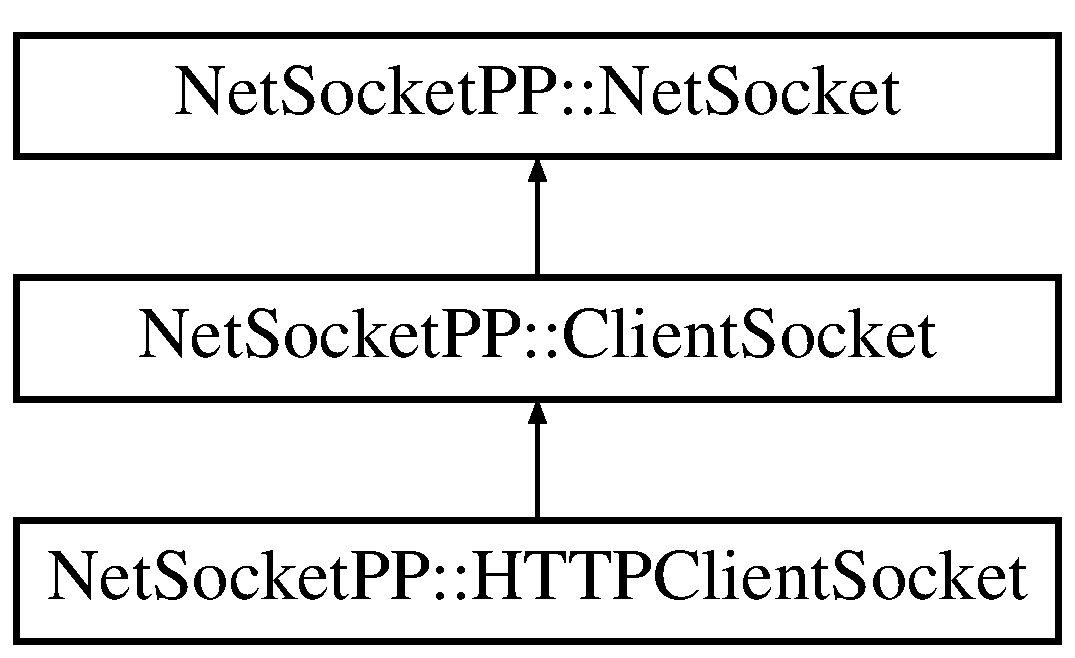
\includegraphics[height=3.000000cm]{class_net_socket_p_p_1_1_client_socket}
\end{center}
\end{figure}
\subsection*{Public Member Functions}
\begin{DoxyCompactItemize}
\item 
\hyperlink{class_net_socket_p_p_1_1_client_socket_a18798784dff930fd46bf9d89c021425f}{Client\-Socket} (std\-::string host, std\-::string service, std\-::string protocol)
\begin{DoxyCompactList}\small\item\em A constructor with parameters, that creates and connects the socket. \end{DoxyCompactList}\item 
int \hyperlink{class_net_socket_p_p_1_1_client_socket_a1317645d6afb05c46abbb3b62e75c86a}{send} (std\-::string msg, int flags)
\begin{DoxyCompactList}\small\item\em A function, that sends data through the socket. \end{DoxyCompactList}\item 
int \hyperlink{class_net_socket_p_p_1_1_client_socket_aa2761de701972e2dbda39919d83c9467}{recv} (int flags)
\begin{DoxyCompactList}\small\item\em A function, that receives data through the socket. \end{DoxyCompactList}\item 
std\-::string \hyperlink{class_net_socket_p_p_1_1_client_socket_ae32fa1faac049522fd1f1f7760936370}{get} ()
\begin{DoxyCompactList}\small\item\em A function returning recently recv-\/d data. \end{DoxyCompactList}\end{DoxyCompactItemize}
\subsection*{Protected Attributes}
\begin{DoxyCompactItemize}
\item 
\hypertarget{class_net_socket_p_p_1_1_client_socket_a8b1405dc86b43d907a6a37d859a3eae9}{char \hyperlink{class_net_socket_p_p_1_1_client_socket_a8b1405dc86b43d907a6a37d859a3eae9}{buf} \mbox{[}100000\mbox{]}}\label{class_net_socket_p_p_1_1_client_socket_a8b1405dc86b43d907a6a37d859a3eae9}

\begin{DoxyCompactList}\small\item\em A large buffer for data. \end{DoxyCompactList}\end{DoxyCompactItemize}
\subsection*{Additional Inherited Members}


\subsection{Detailed Description}
An implementation of a client socket. Inherits from \hyperlink{class_net_socket_p_p_1_1_net_socket}{Net\-Socket}. 

\subsection{Constructor \& Destructor Documentation}
\hypertarget{class_net_socket_p_p_1_1_client_socket_a18798784dff930fd46bf9d89c021425f}{\index{Net\-Socket\-P\-P\-::\-Client\-Socket@{Net\-Socket\-P\-P\-::\-Client\-Socket}!Client\-Socket@{Client\-Socket}}
\index{Client\-Socket@{Client\-Socket}!NetSocketPP::ClientSocket@{Net\-Socket\-P\-P\-::\-Client\-Socket}}
\subsubsection[{Client\-Socket}]{\setlength{\rightskip}{0pt plus 5cm}Client\-Socket\-::\-Client\-Socket (
\begin{DoxyParamCaption}
\item[{std\-::string}]{host, }
\item[{std\-::string}]{service, }
\item[{std\-::string}]{protocol}
\end{DoxyParamCaption}
)}}\label{class_net_socket_p_p_1_1_client_socket_a18798784dff930fd46bf9d89c021425f}


A constructor with parameters, that creates and connects the socket. 


\begin{DoxyParams}{Parameters}
{\em host} & A hostname or I\-P address of socket destination. \\
\hline
{\em service} & A port or service identifier, where socket is to be opened. \\
\hline
{\em protocol} & A protocol of the socket, T\-C\-P or U\-D\-P. \\
\hline
\end{DoxyParams}


\subsection{Member Function Documentation}
\hypertarget{class_net_socket_p_p_1_1_client_socket_ae32fa1faac049522fd1f1f7760936370}{\index{Net\-Socket\-P\-P\-::\-Client\-Socket@{Net\-Socket\-P\-P\-::\-Client\-Socket}!get@{get}}
\index{get@{get}!NetSocketPP::ClientSocket@{Net\-Socket\-P\-P\-::\-Client\-Socket}}
\subsubsection[{get}]{\setlength{\rightskip}{0pt plus 5cm}std\-::string Client\-Socket\-::get (
\begin{DoxyParamCaption}
{}
\end{DoxyParamCaption}
)}}\label{class_net_socket_p_p_1_1_client_socket_ae32fa1faac049522fd1f1f7760936370}


A function returning recently recv-\/d data. 

\begin{DoxyReturn}{Returns}
Received data as std\-::string. 
\end{DoxyReturn}
\hypertarget{class_net_socket_p_p_1_1_client_socket_aa2761de701972e2dbda39919d83c9467}{\index{Net\-Socket\-P\-P\-::\-Client\-Socket@{Net\-Socket\-P\-P\-::\-Client\-Socket}!recv@{recv}}
\index{recv@{recv}!NetSocketPP::ClientSocket@{Net\-Socket\-P\-P\-::\-Client\-Socket}}
\subsubsection[{recv}]{\setlength{\rightskip}{0pt plus 5cm}int Client\-Socket\-::recv (
\begin{DoxyParamCaption}
\item[{int}]{flags}
\end{DoxyParamCaption}
)}}\label{class_net_socket_p_p_1_1_client_socket_aa2761de701972e2dbda39919d83c9467}


A function, that receives data through the socket. 


\begin{DoxyParams}{Parameters}
{\em flags} & Socket flags, default 0. \\
\hline
\end{DoxyParams}
\begin{DoxyReturn}{Returns}
Number of bytes received. 
\end{DoxyReturn}
\hypertarget{class_net_socket_p_p_1_1_client_socket_a1317645d6afb05c46abbb3b62e75c86a}{\index{Net\-Socket\-P\-P\-::\-Client\-Socket@{Net\-Socket\-P\-P\-::\-Client\-Socket}!send@{send}}
\index{send@{send}!NetSocketPP::ClientSocket@{Net\-Socket\-P\-P\-::\-Client\-Socket}}
\subsubsection[{send}]{\setlength{\rightskip}{0pt plus 5cm}int Client\-Socket\-::send (
\begin{DoxyParamCaption}
\item[{std\-::string}]{msg, }
\item[{int}]{flags = {\ttfamily 0}}
\end{DoxyParamCaption}
)}}\label{class_net_socket_p_p_1_1_client_socket_a1317645d6afb05c46abbb3b62e75c86a}


A function, that sends data through the socket. 


\begin{DoxyParams}{Parameters}
{\em msg} & A message to send. \\
\hline
{\em flags} & Socket flags, default 0. \\
\hline
\end{DoxyParams}
\begin{DoxyReturn}{Returns}
Number of bytes sent. 
\end{DoxyReturn}


The documentation for this class was generated from the following files\-:\begin{DoxyCompactItemize}
\item 
\hyperlink{_client_socket_8h}{Client\-Socket.\-h}\item 
Client\-Socket.\-cpp\end{DoxyCompactItemize}

\hypertarget{class_net_socket_p_p_1_1_h_t_t_p_client_socket}{\section{Net\-Socket\-P\-P\-:\-:H\-T\-T\-P\-Client\-Socket Class Reference}
\label{class_net_socket_p_p_1_1_h_t_t_p_client_socket}\index{Net\-Socket\-P\-P\-::\-H\-T\-T\-P\-Client\-Socket@{Net\-Socket\-P\-P\-::\-H\-T\-T\-P\-Client\-Socket}}
}


A class representing H\-T\-T\-P client socket.  




{\ttfamily \#include $<$H\-T\-T\-P\-Client\-Socket.\-h$>$}

Inheritance diagram for Net\-Socket\-P\-P\-:\-:H\-T\-T\-P\-Client\-Socket\-:\begin{figure}[H]
\begin{center}
\leavevmode
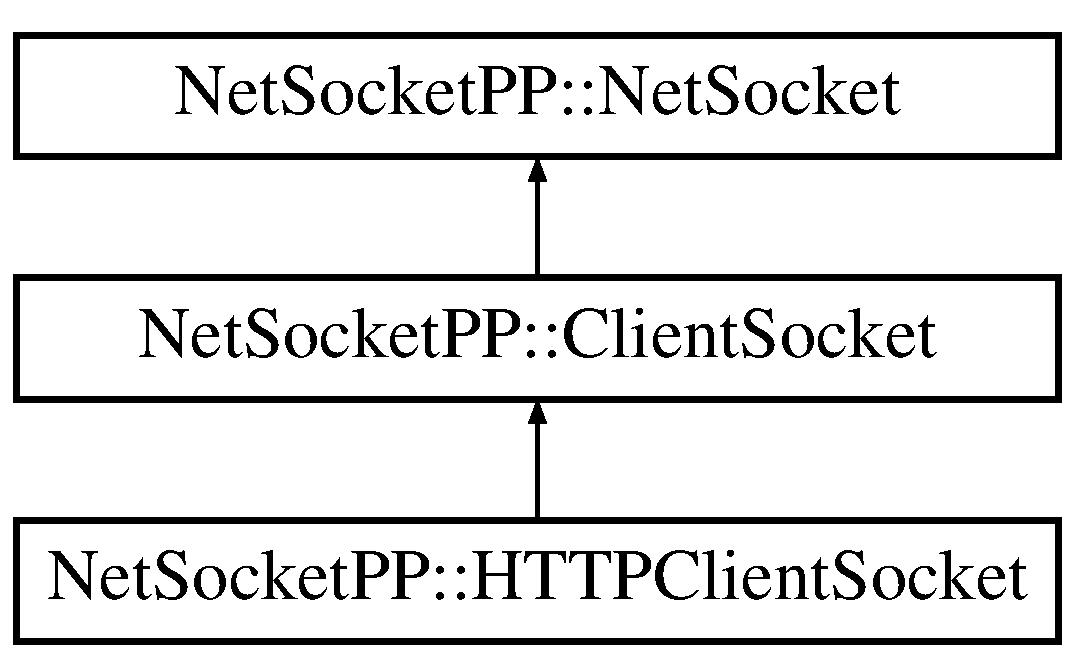
\includegraphics[height=3.000000cm]{class_net_socket_p_p_1_1_h_t_t_p_client_socket}
\end{center}
\end{figure}
\subsection*{Public Member Functions}
\begin{DoxyCompactItemize}
\item 
\hyperlink{class_net_socket_p_p_1_1_h_t_t_p_client_socket_a3512fce741550f229a63d8f6b0914261}{H\-T\-T\-P\-Client\-Socket} (std\-::string host, std\-::string service, std\-::string doc\-Request)
\begin{DoxyCompactList}\small\item\em A constructor with parameters. \end{DoxyCompactList}\item 
\hyperlink{class_net_socket_p_p_1_1_h_t_t_p_reply}{H\-T\-T\-P\-Reply} \hyperlink{class_net_socket_p_p_1_1_h_t_t_p_client_socket_a9693ffad07bdf7916a5dd227146c8bcf}{get\-Reply} ()
\begin{DoxyCompactList}\small\item\em A function returning a \hyperlink{class_net_socket_p_p_1_1_h_t_t_p_reply}{H\-T\-T\-P\-Reply}. \end{DoxyCompactList}\item 
std\-::string \hyperlink{class_net_socket_p_p_1_1_h_t_t_p_client_socket_a710bdbe32e4cdb87b86aa2edd93a1015}{get\-Request} ()
\begin{DoxyCompactList}\small\item\em A function returning the request used in the socket. \end{DoxyCompactList}\end{DoxyCompactItemize}
\subsection*{Additional Inherited Members}


\subsection{Detailed Description}
A class representing H\-T\-T\-P client socket. 

\subsection{Constructor \& Destructor Documentation}
\hypertarget{class_net_socket_p_p_1_1_h_t_t_p_client_socket_a3512fce741550f229a63d8f6b0914261}{\index{Net\-Socket\-P\-P\-::\-H\-T\-T\-P\-Client\-Socket@{Net\-Socket\-P\-P\-::\-H\-T\-T\-P\-Client\-Socket}!H\-T\-T\-P\-Client\-Socket@{H\-T\-T\-P\-Client\-Socket}}
\index{H\-T\-T\-P\-Client\-Socket@{H\-T\-T\-P\-Client\-Socket}!NetSocketPP::HTTPClientSocket@{Net\-Socket\-P\-P\-::\-H\-T\-T\-P\-Client\-Socket}}
\subsubsection[{H\-T\-T\-P\-Client\-Socket}]{\setlength{\rightskip}{0pt plus 5cm}H\-T\-T\-P\-Client\-Socket\-::\-H\-T\-T\-P\-Client\-Socket (
\begin{DoxyParamCaption}
\item[{std\-::string}]{host = {\ttfamily NULL}, }
\item[{std\-::string}]{service = {\ttfamily \char`\"{}http\char`\"{}}, }
\item[{std\-::string}]{doc\-Request = {\ttfamily \char`\"{}/\char`\"{}}}
\end{DoxyParamCaption}
)}}\label{class_net_socket_p_p_1_1_h_t_t_p_client_socket_a3512fce741550f229a63d8f6b0914261}


A constructor with parameters. 


\begin{DoxyParams}{Parameters}
{\em host} & Hostname or I\-P of socket destination, defaults to N\-U\-L\-L. \\
\hline
{\em service} & Service port or identifier, defaults to H\-T\-T\-P. \\
\hline
{\em doc\-Request} & A document to request from the server, defaults to root/index (/). \\
\hline
\end{DoxyParams}


\subsection{Member Function Documentation}
\hypertarget{class_net_socket_p_p_1_1_h_t_t_p_client_socket_a9693ffad07bdf7916a5dd227146c8bcf}{\index{Net\-Socket\-P\-P\-::\-H\-T\-T\-P\-Client\-Socket@{Net\-Socket\-P\-P\-::\-H\-T\-T\-P\-Client\-Socket}!get\-Reply@{get\-Reply}}
\index{get\-Reply@{get\-Reply}!NetSocketPP::HTTPClientSocket@{Net\-Socket\-P\-P\-::\-H\-T\-T\-P\-Client\-Socket}}
\subsubsection[{get\-Reply}]{\setlength{\rightskip}{0pt plus 5cm}{\bf H\-T\-T\-P\-Reply} H\-T\-T\-P\-Client\-Socket\-::get\-Reply (
\begin{DoxyParamCaption}
{}
\end{DoxyParamCaption}
)}}\label{class_net_socket_p_p_1_1_h_t_t_p_client_socket_a9693ffad07bdf7916a5dd227146c8bcf}


A function returning a \hyperlink{class_net_socket_p_p_1_1_h_t_t_p_reply}{H\-T\-T\-P\-Reply}. 

\begin{DoxyReturn}{Returns}
\hyperlink{class_net_socket_p_p_1_1_h_t_t_p_reply}{H\-T\-T\-P\-Reply} object containing received data. 
\end{DoxyReturn}
\hypertarget{class_net_socket_p_p_1_1_h_t_t_p_client_socket_a710bdbe32e4cdb87b86aa2edd93a1015}{\index{Net\-Socket\-P\-P\-::\-H\-T\-T\-P\-Client\-Socket@{Net\-Socket\-P\-P\-::\-H\-T\-T\-P\-Client\-Socket}!get\-Request@{get\-Request}}
\index{get\-Request@{get\-Request}!NetSocketPP::HTTPClientSocket@{Net\-Socket\-P\-P\-::\-H\-T\-T\-P\-Client\-Socket}}
\subsubsection[{get\-Request}]{\setlength{\rightskip}{0pt plus 5cm}std\-::string H\-T\-T\-P\-Client\-Socket\-::get\-Request (
\begin{DoxyParamCaption}
{}
\end{DoxyParamCaption}
)}}\label{class_net_socket_p_p_1_1_h_t_t_p_client_socket_a710bdbe32e4cdb87b86aa2edd93a1015}


A function returning the request used in the socket. 

\begin{DoxyReturn}{Returns}
The H\-T\-T\-P request used to obtain data. 
\end{DoxyReturn}


The documentation for this class was generated from the following files\-:\begin{DoxyCompactItemize}
\item 
\hyperlink{_h_t_t_p_client_socket_8h}{H\-T\-T\-P\-Client\-Socket.\-h}\item 
H\-T\-T\-P\-Client\-Socket.\-cpp\end{DoxyCompactItemize}

\hypertarget{class_net_socket_p_p_1_1_h_t_t_p_reply}{\section{Net\-Socket\-P\-P\-:\-:H\-T\-T\-P\-Reply Class Reference}
\label{class_net_socket_p_p_1_1_h_t_t_p_reply}\index{Net\-Socket\-P\-P\-::\-H\-T\-T\-P\-Reply@{Net\-Socket\-P\-P\-::\-H\-T\-T\-P\-Reply}}
}


A class representing H\-T\-T\-P Reply.  




{\ttfamily \#include $<$H\-T\-T\-P\-Client\-Socket.\-h$>$}

\subsection*{Public Member Functions}
\begin{DoxyCompactItemize}
\item 
\hypertarget{class_net_socket_p_p_1_1_h_t_t_p_reply_acb0b1c18264376e87701488236dce91d}{\hyperlink{class_net_socket_p_p_1_1_h_t_t_p_reply_acb0b1c18264376e87701488236dce91d}{H\-T\-T\-P\-Reply} ()}\label{class_net_socket_p_p_1_1_h_t_t_p_reply_acb0b1c18264376e87701488236dce91d}

\begin{DoxyCompactList}\small\item\em A constructor. \end{DoxyCompactList}\item 
\hyperlink{class_net_socket_p_p_1_1_h_t_t_p_reply_aa75ff9fdbc72fcba9b7c9fb70b3456db}{H\-T\-T\-P\-Reply} (std\-::string raw)
\begin{DoxyCompactList}\small\item\em A constructor with parameter. \end{DoxyCompactList}\item 
\hypertarget{class_net_socket_p_p_1_1_h_t_t_p_reply_a13e1e2f53a1442efd78dbaa3735050ad}{\hyperlink{class_net_socket_p_p_1_1_h_t_t_p_reply_a13e1e2f53a1442efd78dbaa3735050ad}{$\sim$\-H\-T\-T\-P\-Reply} ()}\label{class_net_socket_p_p_1_1_h_t_t_p_reply_a13e1e2f53a1442efd78dbaa3735050ad}

\begin{DoxyCompactList}\small\item\em A destructor. \end{DoxyCompactList}\item 
\hypertarget{class_net_socket_p_p_1_1_h_t_t_p_reply_ad01824f3a3d122869602f38783d29943}{void \hyperlink{class_net_socket_p_p_1_1_h_t_t_p_reply_ad01824f3a3d122869602f38783d29943}{parse} ()}\label{class_net_socket_p_p_1_1_h_t_t_p_reply_ad01824f3a3d122869602f38783d29943}

\begin{DoxyCompactList}\small\item\em H\-T\-T\-P reply parser. \end{DoxyCompactList}\item 
void \hyperlink{class_net_socket_p_p_1_1_h_t_t_p_reply_a07071d35197f3f4217be5b1b330d9e31}{add\-To\-Content} (std\-::string cp)
\begin{DoxyCompactList}\small\item\em A function, that adds more parts of the content to the reply if necessary. \end{DoxyCompactList}\item 
std\-::string \hyperlink{class_net_socket_p_p_1_1_h_t_t_p_reply_a2302029e3b68ae404fc7d0610a119a1e}{get\-Raw} ()
\begin{DoxyCompactList}\small\item\em A function returning raw H\-T\-T\-P reply. \end{DoxyCompactList}\item 
std\-::string \hyperlink{class_net_socket_p_p_1_1_h_t_t_p_reply_a61def153ad4e5ca5a82b9f80eb66a842}{get\-Protocol} ()
\begin{DoxyCompactList}\small\item\em A function returning H\-T\-T\-P protocol information. \end{DoxyCompactList}\item 
std\-::string \hyperlink{class_net_socket_p_p_1_1_h_t_t_p_reply_ab7b23f9fa3ced6d0243a8a9b5d65fb91}{get\-Response} ()
\begin{DoxyCompactList}\small\item\em A function returning H\-T\-T\-P response message. \end{DoxyCompactList}\item 
std\-::string \hyperlink{class_net_socket_p_p_1_1_h_t_t_p_reply_ab0d92359b15b40b1b91305819f16b1f5}{get\-Timestamp} ()
\begin{DoxyCompactList}\small\item\em A function returning timestamp. \end{DoxyCompactList}\item 
std\-::string \hyperlink{class_net_socket_p_p_1_1_h_t_t_p_reply_a57faaec28d71b168af5d7c63b4dce77a}{get\-Server} ()
\begin{DoxyCompactList}\small\item\em A function returning server information. \end{DoxyCompactList}\item 
unsigned int \hyperlink{class_net_socket_p_p_1_1_h_t_t_p_reply_a951724658c775cd639dd869e4cd3ada3}{get\-Content\-Length} ()
\begin{DoxyCompactList}\small\item\em A function returning length of content. \end{DoxyCompactList}\item 
std\-::string \hyperlink{class_net_socket_p_p_1_1_h_t_t_p_reply_a550ee33eceae2f2cfcb650781318da8a}{get\-Connection} ()
\begin{DoxyCompactList}\small\item\em A function returning connection status. \end{DoxyCompactList}\item 
std\-::string \hyperlink{class_net_socket_p_p_1_1_h_t_t_p_reply_a9d19759dc379a7608cf64c8e1150bab4}{get\-Content\-Type} ()
\begin{DoxyCompactList}\small\item\em A function returning type of content. \end{DoxyCompactList}\item 
std\-::string \hyperlink{class_net_socket_p_p_1_1_h_t_t_p_reply_ad307a94f0079131ad25c57bb1851cd32}{get\-Content} ()
\begin{DoxyCompactList}\small\item\em A function returning received content. \end{DoxyCompactList}\end{DoxyCompactItemize}


\subsection{Detailed Description}
A class representing H\-T\-T\-P Reply. 

\subsection{Constructor \& Destructor Documentation}
\hypertarget{class_net_socket_p_p_1_1_h_t_t_p_reply_aa75ff9fdbc72fcba9b7c9fb70b3456db}{\index{Net\-Socket\-P\-P\-::\-H\-T\-T\-P\-Reply@{Net\-Socket\-P\-P\-::\-H\-T\-T\-P\-Reply}!H\-T\-T\-P\-Reply@{H\-T\-T\-P\-Reply}}
\index{H\-T\-T\-P\-Reply@{H\-T\-T\-P\-Reply}!NetSocketPP::HTTPReply@{Net\-Socket\-P\-P\-::\-H\-T\-T\-P\-Reply}}
\subsubsection[{H\-T\-T\-P\-Reply}]{\setlength{\rightskip}{0pt plus 5cm}H\-T\-T\-P\-Reply\-::\-H\-T\-T\-P\-Reply (
\begin{DoxyParamCaption}
\item[{std\-::string}]{raw}
\end{DoxyParamCaption}
)}}\label{class_net_socket_p_p_1_1_h_t_t_p_reply_aa75ff9fdbc72fcba9b7c9fb70b3456db}


A constructor with parameter. 


\begin{DoxyParams}{Parameters}
{\em raw} & Raw reply from recv. \\
\hline
\end{DoxyParams}


\subsection{Member Function Documentation}
\hypertarget{class_net_socket_p_p_1_1_h_t_t_p_reply_a07071d35197f3f4217be5b1b330d9e31}{\index{Net\-Socket\-P\-P\-::\-H\-T\-T\-P\-Reply@{Net\-Socket\-P\-P\-::\-H\-T\-T\-P\-Reply}!add\-To\-Content@{add\-To\-Content}}
\index{add\-To\-Content@{add\-To\-Content}!NetSocketPP::HTTPReply@{Net\-Socket\-P\-P\-::\-H\-T\-T\-P\-Reply}}
\subsubsection[{add\-To\-Content}]{\setlength{\rightskip}{0pt plus 5cm}void H\-T\-T\-P\-Reply\-::add\-To\-Content (
\begin{DoxyParamCaption}
\item[{std\-::string}]{cp}
\end{DoxyParamCaption}
)}}\label{class_net_socket_p_p_1_1_h_t_t_p_reply_a07071d35197f3f4217be5b1b330d9e31}


A function, that adds more parts of the content to the reply if necessary. 


\begin{DoxyParams}{Parameters}
{\em cp} & Part of the content to be added. \\
\hline
\end{DoxyParams}
\hypertarget{class_net_socket_p_p_1_1_h_t_t_p_reply_a550ee33eceae2f2cfcb650781318da8a}{\index{Net\-Socket\-P\-P\-::\-H\-T\-T\-P\-Reply@{Net\-Socket\-P\-P\-::\-H\-T\-T\-P\-Reply}!get\-Connection@{get\-Connection}}
\index{get\-Connection@{get\-Connection}!NetSocketPP::HTTPReply@{Net\-Socket\-P\-P\-::\-H\-T\-T\-P\-Reply}}
\subsubsection[{get\-Connection}]{\setlength{\rightskip}{0pt plus 5cm}std\-::string H\-T\-T\-P\-Reply\-::get\-Connection (
\begin{DoxyParamCaption}
{}
\end{DoxyParamCaption}
)}}\label{class_net_socket_p_p_1_1_h_t_t_p_reply_a550ee33eceae2f2cfcb650781318da8a}


A function returning connection status. 

\begin{DoxyReturn}{Returns}
Connection status. 
\end{DoxyReturn}
\hypertarget{class_net_socket_p_p_1_1_h_t_t_p_reply_ad307a94f0079131ad25c57bb1851cd32}{\index{Net\-Socket\-P\-P\-::\-H\-T\-T\-P\-Reply@{Net\-Socket\-P\-P\-::\-H\-T\-T\-P\-Reply}!get\-Content@{get\-Content}}
\index{get\-Content@{get\-Content}!NetSocketPP::HTTPReply@{Net\-Socket\-P\-P\-::\-H\-T\-T\-P\-Reply}}
\subsubsection[{get\-Content}]{\setlength{\rightskip}{0pt plus 5cm}std\-::string H\-T\-T\-P\-Reply\-::get\-Content (
\begin{DoxyParamCaption}
{}
\end{DoxyParamCaption}
)}}\label{class_net_socket_p_p_1_1_h_t_t_p_reply_ad307a94f0079131ad25c57bb1851cd32}


A function returning received content. 

\begin{DoxyReturn}{Returns}
Received content. 
\end{DoxyReturn}
\hypertarget{class_net_socket_p_p_1_1_h_t_t_p_reply_a951724658c775cd639dd869e4cd3ada3}{\index{Net\-Socket\-P\-P\-::\-H\-T\-T\-P\-Reply@{Net\-Socket\-P\-P\-::\-H\-T\-T\-P\-Reply}!get\-Content\-Length@{get\-Content\-Length}}
\index{get\-Content\-Length@{get\-Content\-Length}!NetSocketPP::HTTPReply@{Net\-Socket\-P\-P\-::\-H\-T\-T\-P\-Reply}}
\subsubsection[{get\-Content\-Length}]{\setlength{\rightskip}{0pt plus 5cm}unsigned int H\-T\-T\-P\-Reply\-::get\-Content\-Length (
\begin{DoxyParamCaption}
{}
\end{DoxyParamCaption}
)}}\label{class_net_socket_p_p_1_1_h_t_t_p_reply_a951724658c775cd639dd869e4cd3ada3}


A function returning length of content. 

\begin{DoxyReturn}{Returns}
Length of content. 
\end{DoxyReturn}
\hypertarget{class_net_socket_p_p_1_1_h_t_t_p_reply_a9d19759dc379a7608cf64c8e1150bab4}{\index{Net\-Socket\-P\-P\-::\-H\-T\-T\-P\-Reply@{Net\-Socket\-P\-P\-::\-H\-T\-T\-P\-Reply}!get\-Content\-Type@{get\-Content\-Type}}
\index{get\-Content\-Type@{get\-Content\-Type}!NetSocketPP::HTTPReply@{Net\-Socket\-P\-P\-::\-H\-T\-T\-P\-Reply}}
\subsubsection[{get\-Content\-Type}]{\setlength{\rightskip}{0pt plus 5cm}std\-::string H\-T\-T\-P\-Reply\-::get\-Content\-Type (
\begin{DoxyParamCaption}
{}
\end{DoxyParamCaption}
)}}\label{class_net_socket_p_p_1_1_h_t_t_p_reply_a9d19759dc379a7608cf64c8e1150bab4}


A function returning type of content. 

\begin{DoxyReturn}{Returns}
Type of content. 
\end{DoxyReturn}
\hypertarget{class_net_socket_p_p_1_1_h_t_t_p_reply_a61def153ad4e5ca5a82b9f80eb66a842}{\index{Net\-Socket\-P\-P\-::\-H\-T\-T\-P\-Reply@{Net\-Socket\-P\-P\-::\-H\-T\-T\-P\-Reply}!get\-Protocol@{get\-Protocol}}
\index{get\-Protocol@{get\-Protocol}!NetSocketPP::HTTPReply@{Net\-Socket\-P\-P\-::\-H\-T\-T\-P\-Reply}}
\subsubsection[{get\-Protocol}]{\setlength{\rightskip}{0pt plus 5cm}std\-::string H\-T\-T\-P\-Reply\-::get\-Protocol (
\begin{DoxyParamCaption}
{}
\end{DoxyParamCaption}
)}}\label{class_net_socket_p_p_1_1_h_t_t_p_reply_a61def153ad4e5ca5a82b9f80eb66a842}


A function returning H\-T\-T\-P protocol information. 

\begin{DoxyReturn}{Returns}
H\-T\-T\-P protocol information. 
\end{DoxyReturn}
\hypertarget{class_net_socket_p_p_1_1_h_t_t_p_reply_a2302029e3b68ae404fc7d0610a119a1e}{\index{Net\-Socket\-P\-P\-::\-H\-T\-T\-P\-Reply@{Net\-Socket\-P\-P\-::\-H\-T\-T\-P\-Reply}!get\-Raw@{get\-Raw}}
\index{get\-Raw@{get\-Raw}!NetSocketPP::HTTPReply@{Net\-Socket\-P\-P\-::\-H\-T\-T\-P\-Reply}}
\subsubsection[{get\-Raw}]{\setlength{\rightskip}{0pt plus 5cm}std\-::string H\-T\-T\-P\-Reply\-::get\-Raw (
\begin{DoxyParamCaption}
{}
\end{DoxyParamCaption}
)}}\label{class_net_socket_p_p_1_1_h_t_t_p_reply_a2302029e3b68ae404fc7d0610a119a1e}


A function returning raw H\-T\-T\-P reply. 

\begin{DoxyReturn}{Returns}
Raw H\-T\-T\-P reply. 
\end{DoxyReturn}
\hypertarget{class_net_socket_p_p_1_1_h_t_t_p_reply_ab7b23f9fa3ced6d0243a8a9b5d65fb91}{\index{Net\-Socket\-P\-P\-::\-H\-T\-T\-P\-Reply@{Net\-Socket\-P\-P\-::\-H\-T\-T\-P\-Reply}!get\-Response@{get\-Response}}
\index{get\-Response@{get\-Response}!NetSocketPP::HTTPReply@{Net\-Socket\-P\-P\-::\-H\-T\-T\-P\-Reply}}
\subsubsection[{get\-Response}]{\setlength{\rightskip}{0pt plus 5cm}std\-::string H\-T\-T\-P\-Reply\-::get\-Response (
\begin{DoxyParamCaption}
{}
\end{DoxyParamCaption}
)}}\label{class_net_socket_p_p_1_1_h_t_t_p_reply_ab7b23f9fa3ced6d0243a8a9b5d65fb91}


A function returning H\-T\-T\-P response message. 

\begin{DoxyReturn}{Returns}
H\-T\-T\-P response message. 
\end{DoxyReturn}
\hypertarget{class_net_socket_p_p_1_1_h_t_t_p_reply_a57faaec28d71b168af5d7c63b4dce77a}{\index{Net\-Socket\-P\-P\-::\-H\-T\-T\-P\-Reply@{Net\-Socket\-P\-P\-::\-H\-T\-T\-P\-Reply}!get\-Server@{get\-Server}}
\index{get\-Server@{get\-Server}!NetSocketPP::HTTPReply@{Net\-Socket\-P\-P\-::\-H\-T\-T\-P\-Reply}}
\subsubsection[{get\-Server}]{\setlength{\rightskip}{0pt plus 5cm}std\-::string H\-T\-T\-P\-Reply\-::get\-Server (
\begin{DoxyParamCaption}
{}
\end{DoxyParamCaption}
)}}\label{class_net_socket_p_p_1_1_h_t_t_p_reply_a57faaec28d71b168af5d7c63b4dce77a}


A function returning server information. 

\begin{DoxyReturn}{Returns}
Server information. 
\end{DoxyReturn}
\hypertarget{class_net_socket_p_p_1_1_h_t_t_p_reply_ab0d92359b15b40b1b91305819f16b1f5}{\index{Net\-Socket\-P\-P\-::\-H\-T\-T\-P\-Reply@{Net\-Socket\-P\-P\-::\-H\-T\-T\-P\-Reply}!get\-Timestamp@{get\-Timestamp}}
\index{get\-Timestamp@{get\-Timestamp}!NetSocketPP::HTTPReply@{Net\-Socket\-P\-P\-::\-H\-T\-T\-P\-Reply}}
\subsubsection[{get\-Timestamp}]{\setlength{\rightskip}{0pt plus 5cm}std\-::string H\-T\-T\-P\-Reply\-::get\-Timestamp (
\begin{DoxyParamCaption}
{}
\end{DoxyParamCaption}
)}}\label{class_net_socket_p_p_1_1_h_t_t_p_reply_ab0d92359b15b40b1b91305819f16b1f5}


A function returning timestamp. 

\begin{DoxyReturn}{Returns}
Timestamp. 
\end{DoxyReturn}


The documentation for this class was generated from the following files\-:\begin{DoxyCompactItemize}
\item 
\hyperlink{_h_t_t_p_client_socket_8h}{H\-T\-T\-P\-Client\-Socket.\-h}\item 
H\-T\-T\-P\-Client\-Socket.\-cpp\end{DoxyCompactItemize}

\hypertarget{class_net_socket_p_p_1_1_net_socket}{\section{Net\-Socket\-P\-P\-:\-:Net\-Socket Class Reference}
\label{class_net_socket_p_p_1_1_net_socket}\index{Net\-Socket\-P\-P\-::\-Net\-Socket@{Net\-Socket\-P\-P\-::\-Net\-Socket}}
}


A class, that represents network connection -\/ socket.  




{\ttfamily \#include $<$Net\-Socket.\-h$>$}

Inheritance diagram for Net\-Socket\-P\-P\-:\-:Net\-Socket\-:\begin{figure}[H]
\begin{center}
\leavevmode
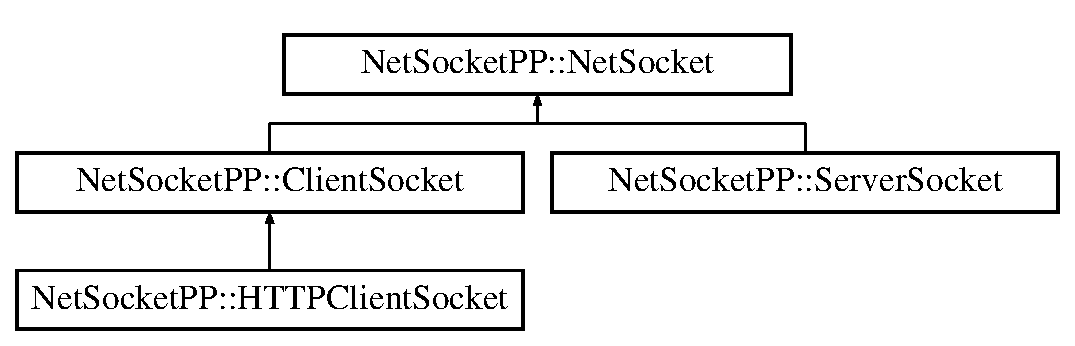
\includegraphics[height=3.000000cm]{class_net_socket_p_p_1_1_net_socket}
\end{center}
\end{figure}
\subsection*{Public Member Functions}
\begin{DoxyCompactItemize}
\item 
\hyperlink{class_net_socket_p_p_1_1_net_socket_abae69a67be7881bbb2fdf605fdd145e5}{Net\-Socket} (std\-::string host, std\-::string service, std\-::string protocol)
\begin{DoxyCompactList}\small\item\em A constructor with parameters, that creates a socket. \end{DoxyCompactList}\item 
std\-::string \hyperlink{class_net_socket_p_p_1_1_net_socket_a3e44de8e02caba69d0763bf7e42c9972}{get\-I\-P} ()
\begin{DoxyCompactList}\small\item\em A function that returns I\-P of a host. \end{DoxyCompactList}\item 
int \hyperlink{class_net_socket_p_p_1_1_net_socket_a932cf37dd25b45aeb9d07439f3fae5a5}{get\-Desc} ()
\begin{DoxyCompactList}\small\item\em A function that returns socket descriptor. \end{DoxyCompactList}\item 
\hypertarget{class_net_socket_p_p_1_1_net_socket_a3ebe4e1d8db6978255f48e1034d638a4}{\hyperlink{class_net_socket_p_p_1_1_net_socket_a3ebe4e1d8db6978255f48e1034d638a4}{$\sim$\-Net\-Socket} ()}\label{class_net_socket_p_p_1_1_net_socket_a3ebe4e1d8db6978255f48e1034d638a4}

\begin{DoxyCompactList}\small\item\em A destructor, that frees the memory. \end{DoxyCompactList}\end{DoxyCompactItemize}
\subsection*{Protected Member Functions}
\begin{DoxyCompactItemize}
\item 
\hypertarget{class_net_socket_p_p_1_1_net_socket_a240ac4d2e384549b5757a79d0e2146bf}{void $\ast$ \hyperlink{class_net_socket_p_p_1_1_net_socket_a240ac4d2e384549b5757a79d0e2146bf}{get\-\_\-in\-\_\-addr} (sockaddr $\ast$sa)}\label{class_net_socket_p_p_1_1_net_socket_a240ac4d2e384549b5757a79d0e2146bf}

\begin{DoxyCompactList}\small\item\em Needed for implementation purposes. \end{DoxyCompactList}\end{DoxyCompactItemize}
\subsection*{Protected Attributes}
\begin{DoxyCompactItemize}
\item 
\hypertarget{class_net_socket_p_p_1_1_net_socket_aae1d9340cd9bacb68f789a86e4d2fe45}{int \hyperlink{class_net_socket_p_p_1_1_net_socket_aae1d9340cd9bacb68f789a86e4d2fe45}{\-\_\-descriptor}}\label{class_net_socket_p_p_1_1_net_socket_aae1d9340cd9bacb68f789a86e4d2fe45}

\begin{DoxyCompactList}\small\item\em Socket descriptor. \end{DoxyCompactList}\item 
\hypertarget{class_net_socket_p_p_1_1_net_socket_a4bbe227dc4bd377397ea684d0d6a501a}{int \hyperlink{class_net_socket_p_p_1_1_net_socket_a4bbe227dc4bd377397ea684d0d6a501a}{\-\_\-yes}}\label{class_net_socket_p_p_1_1_net_socket_a4bbe227dc4bd377397ea684d0d6a501a}

\begin{DoxyCompactList}\small\item\em Needed for implementation purposes. \end{DoxyCompactList}\item 
\hypertarget{class_net_socket_p_p_1_1_net_socket_a3ca9404bfc910697ce6a40afdb2a5d8d}{int \hyperlink{class_net_socket_p_p_1_1_net_socket_a3ca9404bfc910697ce6a40afdb2a5d8d}{\-\_\-status}}\label{class_net_socket_p_p_1_1_net_socket_a3ca9404bfc910697ce6a40afdb2a5d8d}

\begin{DoxyCompactList}\small\item\em Needed for implementation purposes. \end{DoxyCompactList}\item 
\hypertarget{class_net_socket_p_p_1_1_net_socket_a412939af9ba30f042f13621592c59c9f}{char \hyperlink{class_net_socket_p_p_1_1_net_socket_a412939af9ba30f042f13621592c59c9f}{\-\_\-caddr} \mbox{[}I\-N\-E\-T6\-\_\-\-A\-D\-D\-R\-S\-T\-R\-L\-E\-N\mbox{]}}\label{class_net_socket_p_p_1_1_net_socket_a412939af9ba30f042f13621592c59c9f}

\begin{DoxyCompactList}\small\item\em A structure that stores I\-P address. \end{DoxyCompactList}\item 
\hypertarget{class_net_socket_p_p_1_1_net_socket_a51849e8e7d23aa11c9b09eb526656ad1}{addrinfo \hyperlink{class_net_socket_p_p_1_1_net_socket_a51849e8e7d23aa11c9b09eb526656ad1}{\-\_\-hints}}\label{class_net_socket_p_p_1_1_net_socket_a51849e8e7d23aa11c9b09eb526656ad1}

\begin{DoxyCompactList}\small\item\em Needed for implementation purposes. \end{DoxyCompactList}\item 
\hypertarget{class_net_socket_p_p_1_1_net_socket_a000735c5be93aefd3297cd2eb3e55ec0}{addrinfo $\ast$ \hyperlink{class_net_socket_p_p_1_1_net_socket_a000735c5be93aefd3297cd2eb3e55ec0}{\-\_\-servinfo}}\label{class_net_socket_p_p_1_1_net_socket_a000735c5be93aefd3297cd2eb3e55ec0}

\begin{DoxyCompactList}\small\item\em Needed for implementation purposes. \end{DoxyCompactList}\item 
\hypertarget{class_net_socket_p_p_1_1_net_socket_aa608f4ab4af1be3c36831f4c0dd386cf}{sockaddr\-\_\-storage \hyperlink{class_net_socket_p_p_1_1_net_socket_aa608f4ab4af1be3c36831f4c0dd386cf}{\-\_\-their\-\_\-addr}}\label{class_net_socket_p_p_1_1_net_socket_aa608f4ab4af1be3c36831f4c0dd386cf}

\begin{DoxyCompactList}\small\item\em Needed for implementation purposes. \end{DoxyCompactList}\item 
\hypertarget{class_net_socket_p_p_1_1_net_socket_a8a19d20260ef37d1adbb7439a55b2b6a}{socklen\-\_\-t \hyperlink{class_net_socket_p_p_1_1_net_socket_a8a19d20260ef37d1adbb7439a55b2b6a}{\-\_\-addr\-\_\-size}}\label{class_net_socket_p_p_1_1_net_socket_a8a19d20260ef37d1adbb7439a55b2b6a}

\begin{DoxyCompactList}\small\item\em Needed for implementation purposes. \end{DoxyCompactList}\item 
\hypertarget{class_net_socket_p_p_1_1_net_socket_ad22749418d441f69226894af0f8467c5}{std\-::string \hyperlink{class_net_socket_p_p_1_1_net_socket_ad22749418d441f69226894af0f8467c5}{\-\_\-host}}\label{class_net_socket_p_p_1_1_net_socket_ad22749418d441f69226894af0f8467c5}

\begin{DoxyCompactList}\small\item\em A host to which a socket is connecting to/on which a server socket is opened. \end{DoxyCompactList}\item 
\hypertarget{class_net_socket_p_p_1_1_net_socket_a2db5c2f404edb3282384529e19ebe173}{std\-::string \hyperlink{class_net_socket_p_p_1_1_net_socket_a2db5c2f404edb3282384529e19ebe173}{\-\_\-service}}\label{class_net_socket_p_p_1_1_net_socket_a2db5c2f404edb3282384529e19ebe173}

\begin{DoxyCompactList}\small\item\em A port or a string identyfing service that socket is connecting to/which server is being opened. \end{DoxyCompactList}\item 
\hypertarget{class_net_socket_p_p_1_1_net_socket_a69be87c77c9cdd187ec59e071cbbd431}{std\-::string \hyperlink{class_net_socket_p_p_1_1_net_socket_a69be87c77c9cdd187ec59e071cbbd431}{\-\_\-protocol}}\label{class_net_socket_p_p_1_1_net_socket_a69be87c77c9cdd187ec59e071cbbd431}

\begin{DoxyCompactList}\small\item\em A protocol of the socket\-: T\-C\-P/\-U\-D\-P. \end{DoxyCompactList}\end{DoxyCompactItemize}


\subsection{Detailed Description}
A class, that represents network connection -\/ socket. 

\subsection{Constructor \& Destructor Documentation}
\hypertarget{class_net_socket_p_p_1_1_net_socket_abae69a67be7881bbb2fdf605fdd145e5}{\index{Net\-Socket\-P\-P\-::\-Net\-Socket@{Net\-Socket\-P\-P\-::\-Net\-Socket}!Net\-Socket@{Net\-Socket}}
\index{Net\-Socket@{Net\-Socket}!NetSocketPP::NetSocket@{Net\-Socket\-P\-P\-::\-Net\-Socket}}
\subsubsection[{Net\-Socket}]{\setlength{\rightskip}{0pt plus 5cm}Net\-Socket\-::\-Net\-Socket (
\begin{DoxyParamCaption}
\item[{std\-::string}]{host, }
\item[{std\-::string}]{service, }
\item[{std\-::string}]{protocol}
\end{DoxyParamCaption}
)}}\label{class_net_socket_p_p_1_1_net_socket_abae69a67be7881bbb2fdf605fdd145e5}


A constructor with parameters, that creates a socket. 


\begin{DoxyParams}{Parameters}
{\em host} & A hostname or I\-P address of socket destination. \\
\hline
{\em service} & A port or service identifier, where socket is to be opened. \\
\hline
{\em protocol} & A protocol of the socket, T\-C\-P or U\-D\-P. \\
\hline
\end{DoxyParams}


\subsection{Member Function Documentation}
\hypertarget{class_net_socket_p_p_1_1_net_socket_a932cf37dd25b45aeb9d07439f3fae5a5}{\index{Net\-Socket\-P\-P\-::\-Net\-Socket@{Net\-Socket\-P\-P\-::\-Net\-Socket}!get\-Desc@{get\-Desc}}
\index{get\-Desc@{get\-Desc}!NetSocketPP::NetSocket@{Net\-Socket\-P\-P\-::\-Net\-Socket}}
\subsubsection[{get\-Desc}]{\setlength{\rightskip}{0pt plus 5cm}int Net\-Socket\-::get\-Desc (
\begin{DoxyParamCaption}
{}
\end{DoxyParamCaption}
)}}\label{class_net_socket_p_p_1_1_net_socket_a932cf37dd25b45aeb9d07439f3fae5a5}


A function that returns socket descriptor. 

\begin{DoxyReturn}{Returns}
A socket descriptor. 
\end{DoxyReturn}
\hypertarget{class_net_socket_p_p_1_1_net_socket_a3e44de8e02caba69d0763bf7e42c9972}{\index{Net\-Socket\-P\-P\-::\-Net\-Socket@{Net\-Socket\-P\-P\-::\-Net\-Socket}!get\-I\-P@{get\-I\-P}}
\index{get\-I\-P@{get\-I\-P}!NetSocketPP::NetSocket@{Net\-Socket\-P\-P\-::\-Net\-Socket}}
\subsubsection[{get\-I\-P}]{\setlength{\rightskip}{0pt plus 5cm}std\-::string Net\-Socket\-::get\-I\-P (
\begin{DoxyParamCaption}
{}
\end{DoxyParamCaption}
)}}\label{class_net_socket_p_p_1_1_net_socket_a3e44de8e02caba69d0763bf7e42c9972}


A function that returns I\-P of a host. 

\begin{DoxyReturn}{Returns}
I\-P address of a host as std\-::string. 
\end{DoxyReturn}


The documentation for this class was generated from the following files\-:\begin{DoxyCompactItemize}
\item 
\hyperlink{_net_socket_8h}{Net\-Socket.\-h}\item 
Net\-Socket.\-cpp\end{DoxyCompactItemize}

\hypertarget{class_net_socket_p_p_1_1_network_exception}{\section{Net\-Socket\-P\-P\-:\-:Network\-Exception Class Reference}
\label{class_net_socket_p_p_1_1_network_exception}\index{Net\-Socket\-P\-P\-::\-Network\-Exception@{Net\-Socket\-P\-P\-::\-Network\-Exception}}
}


A class representing an exception with network.  




{\ttfamily \#include $<$Network\-Exception.\-h$>$}

Inheritance diagram for Net\-Socket\-P\-P\-:\-:Network\-Exception\-:\begin{figure}[H]
\begin{center}
\leavevmode
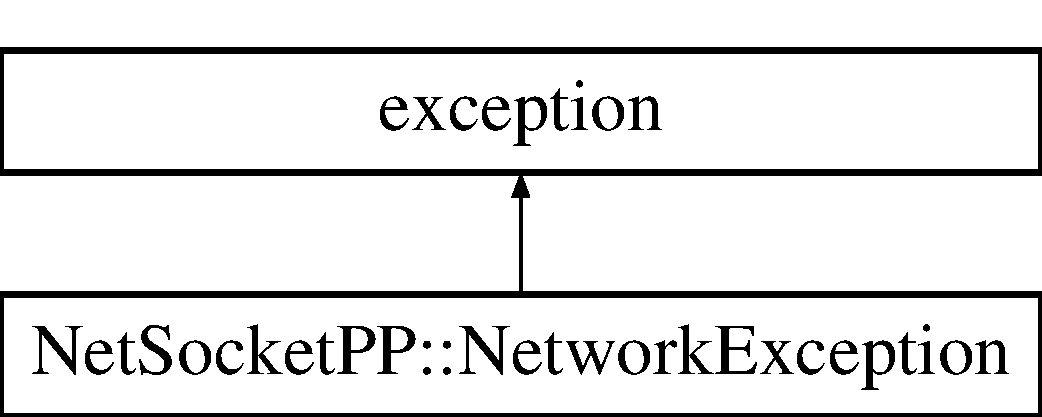
\includegraphics[height=2.000000cm]{class_net_socket_p_p_1_1_network_exception}
\end{center}
\end{figure}
\subsection*{Public Member Functions}
\begin{DoxyCompactItemize}
\item 
\hyperlink{class_net_socket_p_p_1_1_network_exception_a94885d8a86f44db4b88aa5555c38522a}{Network\-Exception} (std\-::string cmd, std\-::string msg)
\begin{DoxyCompactList}\small\item\em A constructor with parameters. \end{DoxyCompactList}\item 
\hypertarget{class_net_socket_p_p_1_1_network_exception_aa47fb62f0baafdc4c158757f533a0d55}{\hyperlink{class_net_socket_p_p_1_1_network_exception_aa47fb62f0baafdc4c158757f533a0d55}{$\sim$\-Network\-Exception} ()  throw ()}\label{class_net_socket_p_p_1_1_network_exception_aa47fb62f0baafdc4c158757f533a0d55}

\begin{DoxyCompactList}\small\item\em A destructor, as needed by std\-::exception. \end{DoxyCompactList}\item 
const char $\ast$ \hyperlink{class_net_socket_p_p_1_1_network_exception_a1ad0c99178e80ffb1432a7a3804cbd05}{what} () const   throw ()
\begin{DoxyCompactList}\small\item\em A function, that returns error message, as needed by std\-::exception. \end{DoxyCompactList}\end{DoxyCompactItemize}


\subsection{Detailed Description}
A class representing an exception with network. 

\subsection{Constructor \& Destructor Documentation}
\hypertarget{class_net_socket_p_p_1_1_network_exception_a94885d8a86f44db4b88aa5555c38522a}{\index{Net\-Socket\-P\-P\-::\-Network\-Exception@{Net\-Socket\-P\-P\-::\-Network\-Exception}!Network\-Exception@{Network\-Exception}}
\index{Network\-Exception@{Network\-Exception}!NetSocketPP::NetworkException@{Net\-Socket\-P\-P\-::\-Network\-Exception}}
\subsubsection[{Network\-Exception}]{\setlength{\rightskip}{0pt plus 5cm}Network\-Exception\-::\-Network\-Exception (
\begin{DoxyParamCaption}
\item[{std\-::string}]{cmd, }
\item[{std\-::string}]{msg}
\end{DoxyParamCaption}
)}}\label{class_net_socket_p_p_1_1_network_exception_a94885d8a86f44db4b88aa5555c38522a}


A constructor with parameters. 


\begin{DoxyParams}{Parameters}
{\em cmd} & A command, where exception occured. \\
\hline
{\em msg} & What has happened. \\
\hline
\end{DoxyParams}


\subsection{Member Function Documentation}
\hypertarget{class_net_socket_p_p_1_1_network_exception_a1ad0c99178e80ffb1432a7a3804cbd05}{\index{Net\-Socket\-P\-P\-::\-Network\-Exception@{Net\-Socket\-P\-P\-::\-Network\-Exception}!what@{what}}
\index{what@{what}!NetSocketPP::NetworkException@{Net\-Socket\-P\-P\-::\-Network\-Exception}}
\subsubsection[{what}]{\setlength{\rightskip}{0pt plus 5cm}const char $\ast$ Network\-Exception\-::what (
\begin{DoxyParamCaption}
{}
\end{DoxyParamCaption}
) const  throw ()}}\label{class_net_socket_p_p_1_1_network_exception_a1ad0c99178e80ffb1432a7a3804cbd05}


A function, that returns error message, as needed by std\-::exception. 

\begin{DoxyReturn}{Returns}
Error message. 
\end{DoxyReturn}


The documentation for this class was generated from the following files\-:\begin{DoxyCompactItemize}
\item 
\hyperlink{_network_exception_8h}{Network\-Exception.\-h}\item 
Network\-Exception.\-cpp\end{DoxyCompactItemize}

\hypertarget{class_net_socket_p_p_1_1_server_function_args}{\section{Net\-Socket\-P\-P\-:\-:Server\-Function\-Args Class Reference}
\label{class_net_socket_p_p_1_1_server_function_args}\index{Net\-Socket\-P\-P\-::\-Server\-Function\-Args@{Net\-Socket\-P\-P\-::\-Server\-Function\-Args}}
}


A class for storing server function arguments.  




{\ttfamily \#include $<$Server\-Socket.\-h$>$}

\subsection*{Public Member Functions}
\begin{DoxyCompactItemize}
\item 
\hypertarget{class_net_socket_p_p_1_1_server_function_args_a12a15c962ca5f38701e8d3f461623668}{\hyperlink{class_net_socket_p_p_1_1_server_function_args_a12a15c962ca5f38701e8d3f461623668}{Server\-Function\-Args} ()}\label{class_net_socket_p_p_1_1_server_function_args_a12a15c962ca5f38701e8d3f461623668}

\begin{DoxyCompactList}\small\item\em A constructor. \end{DoxyCompactList}\item 
\hyperlink{class_net_socket_p_p_1_1_server_function_args_ac7f9a434d7525e09f9568a3b7fb33d51}{Server\-Function\-Args} (\hyperlink{class_net_socket_p_p_1_1_server_function_args}{Server\-Function\-Args} \&sfa)
\begin{DoxyCompactList}\small\item\em A copy constructor. \end{DoxyCompactList}\item 
\hypertarget{class_net_socket_p_p_1_1_server_function_args_a94b84df8925528f994cff8d5f95b56b3}{\hyperlink{class_net_socket_p_p_1_1_server_function_args_a94b84df8925528f994cff8d5f95b56b3}{$\sim$\-Server\-Function\-Args} ()}\label{class_net_socket_p_p_1_1_server_function_args_a94b84df8925528f994cff8d5f95b56b3}

\begin{DoxyCompactList}\small\item\em A destructor. \end{DoxyCompactList}\item 
void \hyperlink{class_net_socket_p_p_1_1_server_function_args_a59fd11d1cef4e1be812da1e2d3399327}{add\-Argument} (std\-::string arg)
\begin{DoxyCompactList}\small\item\em Function adding an argument to the list. \end{DoxyCompactList}\item 
std\-::string \hyperlink{class_net_socket_p_p_1_1_server_function_args_aaf399ccff87f5692d31f7edeb8469e0e}{get\-Argument} (unsigned int idx)
\begin{DoxyCompactList}\small\item\em Function returning the argument of given index number. \end{DoxyCompactList}\item 
std\-::string \hyperlink{class_net_socket_p_p_1_1_server_function_args_a905fd5c411969f8976541a10c243fc40}{operator\mbox{[}$\,$\mbox{]}} (unsigned int idx)
\begin{DoxyCompactList}\small\item\em Operator\mbox{[}\mbox{]} returning the argument of given index number. \end{DoxyCompactList}\end{DoxyCompactItemize}


\subsection{Detailed Description}
A class for storing server function arguments. 

\subsection{Constructor \& Destructor Documentation}
\hypertarget{class_net_socket_p_p_1_1_server_function_args_ac7f9a434d7525e09f9568a3b7fb33d51}{\index{Net\-Socket\-P\-P\-::\-Server\-Function\-Args@{Net\-Socket\-P\-P\-::\-Server\-Function\-Args}!Server\-Function\-Args@{Server\-Function\-Args}}
\index{Server\-Function\-Args@{Server\-Function\-Args}!NetSocketPP::ServerFunctionArgs@{Net\-Socket\-P\-P\-::\-Server\-Function\-Args}}
\subsubsection[{Server\-Function\-Args}]{\setlength{\rightskip}{0pt plus 5cm}Server\-Function\-Args\-::\-Server\-Function\-Args (
\begin{DoxyParamCaption}
\item[{{\bf Server\-Function\-Args} \&}]{sfa}
\end{DoxyParamCaption}
)}}\label{class_net_socket_p_p_1_1_server_function_args_ac7f9a434d7525e09f9568a3b7fb33d51}


A copy constructor. 


\begin{DoxyParams}{Parameters}
{\em sfa} & An object to be copied. \\
\hline
\end{DoxyParams}


\subsection{Member Function Documentation}
\hypertarget{class_net_socket_p_p_1_1_server_function_args_a59fd11d1cef4e1be812da1e2d3399327}{\index{Net\-Socket\-P\-P\-::\-Server\-Function\-Args@{Net\-Socket\-P\-P\-::\-Server\-Function\-Args}!add\-Argument@{add\-Argument}}
\index{add\-Argument@{add\-Argument}!NetSocketPP::ServerFunctionArgs@{Net\-Socket\-P\-P\-::\-Server\-Function\-Args}}
\subsubsection[{add\-Argument}]{\setlength{\rightskip}{0pt plus 5cm}void Server\-Function\-Args\-::add\-Argument (
\begin{DoxyParamCaption}
\item[{std\-::string}]{arg}
\end{DoxyParamCaption}
)}}\label{class_net_socket_p_p_1_1_server_function_args_a59fd11d1cef4e1be812da1e2d3399327}


Function adding an argument to the list. 


\begin{DoxyParams}{Parameters}
{\em arg} & An argument to be added, of type std\-::string. \\
\hline
\end{DoxyParams}
\hypertarget{class_net_socket_p_p_1_1_server_function_args_aaf399ccff87f5692d31f7edeb8469e0e}{\index{Net\-Socket\-P\-P\-::\-Server\-Function\-Args@{Net\-Socket\-P\-P\-::\-Server\-Function\-Args}!get\-Argument@{get\-Argument}}
\index{get\-Argument@{get\-Argument}!NetSocketPP::ServerFunctionArgs@{Net\-Socket\-P\-P\-::\-Server\-Function\-Args}}
\subsubsection[{get\-Argument}]{\setlength{\rightskip}{0pt plus 5cm}std\-::string Server\-Function\-Args\-::get\-Argument (
\begin{DoxyParamCaption}
\item[{unsigned int}]{idx}
\end{DoxyParamCaption}
)}}\label{class_net_socket_p_p_1_1_server_function_args_aaf399ccff87f5692d31f7edeb8469e0e}


Function returning the argument of given index number. 


\begin{DoxyParams}{Parameters}
{\em idx} & Index of the argument. \\
\hline
\end{DoxyParams}
\begin{DoxyReturn}{Returns}
The argument. 
\end{DoxyReturn}
\hypertarget{class_net_socket_p_p_1_1_server_function_args_a905fd5c411969f8976541a10c243fc40}{\index{Net\-Socket\-P\-P\-::\-Server\-Function\-Args@{Net\-Socket\-P\-P\-::\-Server\-Function\-Args}!operator\mbox{[}$\,$\mbox{]}@{operator[]}}
\index{operator\mbox{[}$\,$\mbox{]}@{operator[]}!NetSocketPP::ServerFunctionArgs@{Net\-Socket\-P\-P\-::\-Server\-Function\-Args}}
\subsubsection[{operator[]}]{\setlength{\rightskip}{0pt plus 5cm}std\-::string Server\-Function\-Args\-::operator\mbox{[}$\,$\mbox{]} (
\begin{DoxyParamCaption}
\item[{unsigned int}]{idx}
\end{DoxyParamCaption}
)}}\label{class_net_socket_p_p_1_1_server_function_args_a905fd5c411969f8976541a10c243fc40}


Operator\mbox{[}\mbox{]} returning the argument of given index number. 


\begin{DoxyParams}{Parameters}
{\em idx} & Index of the argument. \\
\hline
\end{DoxyParams}
\begin{DoxyReturn}{Returns}
The argument. 
\end{DoxyReturn}


The documentation for this class was generated from the following files\-:\begin{DoxyCompactItemize}
\item 
\hyperlink{_server_socket_8h}{Server\-Socket.\-h}\item 
Server\-Socket.\-cpp\end{DoxyCompactItemize}

\hypertarget{class_net_socket_p_p_1_1_server_socket}{\section{Net\-Socket\-P\-P\-:\-:Server\-Socket Class Reference}
\label{class_net_socket_p_p_1_1_server_socket}\index{Net\-Socket\-P\-P\-::\-Server\-Socket@{Net\-Socket\-P\-P\-::\-Server\-Socket}}
}


An implementation of the server socket.  




{\ttfamily \#include $<$Server\-Socket.\-h$>$}

Inheritance diagram for Net\-Socket\-P\-P\-:\-:Server\-Socket\-:\begin{figure}[H]
\begin{center}
\leavevmode
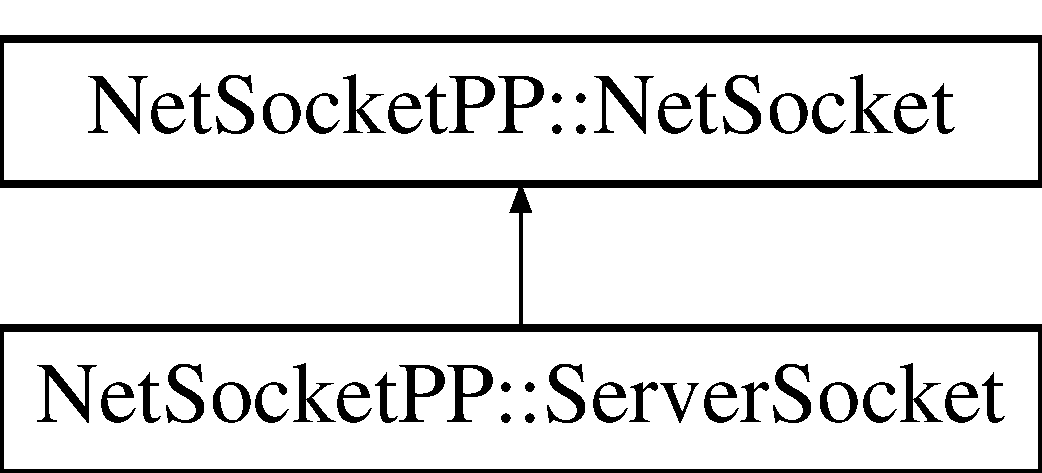
\includegraphics[height=2.000000cm]{class_net_socket_p_p_1_1_server_socket}
\end{center}
\end{figure}
\subsection*{Public Member Functions}
\begin{DoxyCompactItemize}
\item 
\hyperlink{class_net_socket_p_p_1_1_server_socket_a79fb1d52a8dfedaa7f58f904d38d68c0}{Server\-Socket} (std\-::string host, std\-::string service, std\-::string protocol)
\begin{DoxyCompactList}\small\item\em A constructor with parameters. \end{DoxyCompactList}\item 
\hypertarget{class_net_socket_p_p_1_1_server_socket_a510674d924c2544e6b0069e39c36516b}{\hyperlink{class_net_socket_p_p_1_1_server_socket_a510674d924c2544e6b0069e39c36516b}{$\sim$\-Server\-Socket} ()}\label{class_net_socket_p_p_1_1_server_socket_a510674d924c2544e6b0069e39c36516b}

\begin{DoxyCompactList}\small\item\em A destructor. \end{DoxyCompactList}\item 
void \hyperlink{class_net_socket_p_p_1_1_server_socket_a51754d1c346300072a94f4b392a87d38}{start\-Server} (\hyperlink{class_net_socket_p_p_1_1_server_function_args}{Server\-Function\-Args} \&function\-Output, \hyperlink{class_net_socket_p_p_1_1_server_function_args}{Server\-Function\-Args} \&($\ast$server\-Main)(\hyperlink{class_net_socket_p_p_1_1_server_function_args}{Server\-Function\-Args}, \hyperlink{class_net_socket_p_p_1_1_server_socket}{Server\-Socket} $\ast$), \hyperlink{class_net_socket_p_p_1_1_server_function_args}{Server\-Function\-Args} function\-Input, bool infinite, unsigned int iternum, int connection\-Limit)
\begin{DoxyCompactList}\small\item\em A function that starts T\-C\-P server. \end{DoxyCompactList}\item 
int \hyperlink{class_net_socket_p_p_1_1_server_socket_a8bd2cc82d02a5997119b6abdc9d2f1a9}{send} (std\-::string msg, int flags=0)
\begin{DoxyCompactList}\small\item\em A function that sends data through the socket. \end{DoxyCompactList}\item 
int \hyperlink{class_net_socket_p_p_1_1_server_socket_a2e0203c59bfa247f0252e6e13064c6af}{recv} (int flags=0)
\begin{DoxyCompactList}\small\item\em A function that receives data through the socket. \end{DoxyCompactList}\item 
std\-::string \hyperlink{class_net_socket_p_p_1_1_server_socket_a94e3eddcfdb2f04d8f30fb50006d0515}{get} ()
\begin{DoxyCompactList}\small\item\em A function returning received data. \end{DoxyCompactList}\end{DoxyCompactItemize}
\subsection*{Additional Inherited Members}


\subsection{Detailed Description}
An implementation of the server socket. 

\subsection{Constructor \& Destructor Documentation}
\hypertarget{class_net_socket_p_p_1_1_server_socket_a79fb1d52a8dfedaa7f58f904d38d68c0}{\index{Net\-Socket\-P\-P\-::\-Server\-Socket@{Net\-Socket\-P\-P\-::\-Server\-Socket}!Server\-Socket@{Server\-Socket}}
\index{Server\-Socket@{Server\-Socket}!NetSocketPP::ServerSocket@{Net\-Socket\-P\-P\-::\-Server\-Socket}}
\subsubsection[{Server\-Socket}]{\setlength{\rightskip}{0pt plus 5cm}Server\-Socket\-::\-Server\-Socket (
\begin{DoxyParamCaption}
\item[{std\-::string}]{host, }
\item[{std\-::string}]{service, }
\item[{std\-::string}]{protocol}
\end{DoxyParamCaption}
)}}\label{class_net_socket_p_p_1_1_server_socket_a79fb1d52a8dfedaa7f58f904d38d68c0}


A constructor with parameters. 


\begin{DoxyParams}{Parameters}
{\em host} & A hostname or I\-P adress of socket destination, defaults to N\-U\-L\-L. \\
\hline
{\em service} & Port or service that socket should be connected with. \\
\hline
{\em protocol} & Socket protocol, T\-C\-P or U\-D\-P. \\
\hline
\end{DoxyParams}


\subsection{Member Function Documentation}
\hypertarget{class_net_socket_p_p_1_1_server_socket_a94e3eddcfdb2f04d8f30fb50006d0515}{\index{Net\-Socket\-P\-P\-::\-Server\-Socket@{Net\-Socket\-P\-P\-::\-Server\-Socket}!get@{get}}
\index{get@{get}!NetSocketPP::ServerSocket@{Net\-Socket\-P\-P\-::\-Server\-Socket}}
\subsubsection[{get}]{\setlength{\rightskip}{0pt plus 5cm}std\-::string Server\-Socket\-::get (
\begin{DoxyParamCaption}
{}
\end{DoxyParamCaption}
)}}\label{class_net_socket_p_p_1_1_server_socket_a94e3eddcfdb2f04d8f30fb50006d0515}


A function returning received data. 

\begin{DoxyReturn}{Returns}
Received data as string. 
\end{DoxyReturn}
\hypertarget{class_net_socket_p_p_1_1_server_socket_a2e0203c59bfa247f0252e6e13064c6af}{\index{Net\-Socket\-P\-P\-::\-Server\-Socket@{Net\-Socket\-P\-P\-::\-Server\-Socket}!recv@{recv}}
\index{recv@{recv}!NetSocketPP::ServerSocket@{Net\-Socket\-P\-P\-::\-Server\-Socket}}
\subsubsection[{recv}]{\setlength{\rightskip}{0pt plus 5cm}int Server\-Socket\-::recv (
\begin{DoxyParamCaption}
\item[{int}]{flags = {\ttfamily 0}}
\end{DoxyParamCaption}
)}}\label{class_net_socket_p_p_1_1_server_socket_a2e0203c59bfa247f0252e6e13064c6af}


A function that receives data through the socket. 


\begin{DoxyParams}{Parameters}
{\em flags} & Receive flags, defaulting to 0. \\
\hline
\end{DoxyParams}
\begin{DoxyReturn}{Returns}
Number of bytes received. 
\end{DoxyReturn}
\hypertarget{class_net_socket_p_p_1_1_server_socket_a8bd2cc82d02a5997119b6abdc9d2f1a9}{\index{Net\-Socket\-P\-P\-::\-Server\-Socket@{Net\-Socket\-P\-P\-::\-Server\-Socket}!send@{send}}
\index{send@{send}!NetSocketPP::ServerSocket@{Net\-Socket\-P\-P\-::\-Server\-Socket}}
\subsubsection[{send}]{\setlength{\rightskip}{0pt plus 5cm}int Server\-Socket\-::send (
\begin{DoxyParamCaption}
\item[{std\-::string}]{msg, }
\item[{int}]{flags = {\ttfamily 0}}
\end{DoxyParamCaption}
)}}\label{class_net_socket_p_p_1_1_server_socket_a8bd2cc82d02a5997119b6abdc9d2f1a9}


A function that sends data through the socket. 


\begin{DoxyParams}{Parameters}
{\em msg} & A message/data to send, of type std\-::string. \\
\hline
{\em flags} & Send flags, defaulting to 0. \\
\hline
\end{DoxyParams}
\begin{DoxyReturn}{Returns}
Number of bytes sent. 
\end{DoxyReturn}
\hypertarget{class_net_socket_p_p_1_1_server_socket_a51754d1c346300072a94f4b392a87d38}{\index{Net\-Socket\-P\-P\-::\-Server\-Socket@{Net\-Socket\-P\-P\-::\-Server\-Socket}!start\-Server@{start\-Server}}
\index{start\-Server@{start\-Server}!NetSocketPP::ServerSocket@{Net\-Socket\-P\-P\-::\-Server\-Socket}}
\subsubsection[{start\-Server}]{\setlength{\rightskip}{0pt plus 5cm}void Server\-Socket\-::start\-Server (
\begin{DoxyParamCaption}
\item[{{\bf Server\-Function\-Args} \&}]{function\-Output, }
\item[{{\bf Server\-Function\-Args} \&($\ast$)({\bf Server\-Function\-Args}, {\bf Server\-Socket} $\ast$)}]{server\-Main, }
\item[{{\bf Server\-Function\-Args}}]{function\-Input, }
\item[{bool}]{infinite, }
\item[{unsigned int}]{iternum, }
\item[{int}]{connection\-Limit}
\end{DoxyParamCaption}
)}}\label{class_net_socket_p_p_1_1_server_socket_a51754d1c346300072a94f4b392a87d38}


A function that starts T\-C\-P server. 


\begin{DoxyParams}{Parameters}
{\em function\-Output} & A \hyperlink{class_net_socket_p_p_1_1_server_function_args}{Server\-Function\-Args} object that will store server function result. \\
\hline
{\em server\-Main} & An user-\/defined function, that returns \hyperlink{class_net_socket_p_p_1_1_server_function_args}{Server\-Function\-Args} object -\/ results of the server function with arguments\-: \hyperlink{class_net_socket_p_p_1_1_server_function_args}{Server\-Function\-Args} object -\/ arguments to the server function and pointer to \hyperlink{class_net_socket_p_p_1_1_server_socket}{Server\-Socket} object -\/ for passing socket information in that order. \\
\hline
{\em function\-Input} & A \hyperlink{class_net_socket_p_p_1_1_server_function_args}{Server\-Function\-Args} object with server function arguments. \\
\hline
{\em infinite} & Determines if server loop should be infinite. \\
\hline
{\em iternum} & Number of accept() iterations for non-\/infinite loops. \\
\hline
{\em connection\-Limit} & Maximum number of accepted connections. \\
\hline
\end{DoxyParams}


The documentation for this class was generated from the following files\-:\begin{DoxyCompactItemize}
\item 
\hyperlink{_server_socket_8h}{Server\-Socket.\-h}\item 
Server\-Socket.\-cpp\end{DoxyCompactItemize}

\hypertarget{class_net_socket_p_p_1_1_socket_exception}{\section{Net\-Socket\-P\-P\-:\-:Socket\-Exception Class Reference}
\label{class_net_socket_p_p_1_1_socket_exception}\index{Net\-Socket\-P\-P\-::\-Socket\-Exception@{Net\-Socket\-P\-P\-::\-Socket\-Exception}}
}


A class representing an exception with socket classes.  




{\ttfamily \#include $<$Socket\-Exception.\-h$>$}

Inheritance diagram for Net\-Socket\-P\-P\-:\-:Socket\-Exception\-:\begin{figure}[H]
\begin{center}
\leavevmode
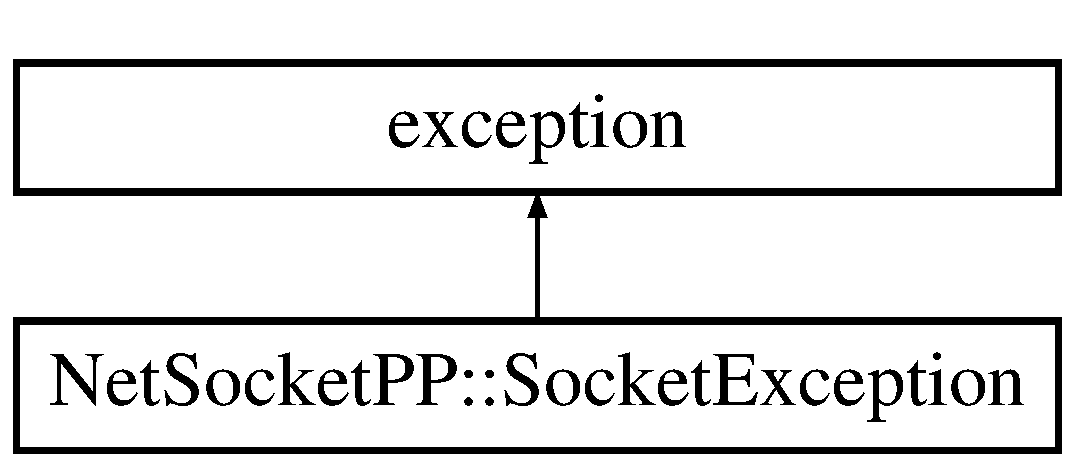
\includegraphics[height=2.000000cm]{class_net_socket_p_p_1_1_socket_exception}
\end{center}
\end{figure}
\subsection*{Public Member Functions}
\begin{DoxyCompactItemize}
\item 
\hyperlink{class_net_socket_p_p_1_1_socket_exception_a7fe2e86c1775289a581156141ec3fb38}{Socket\-Exception} (std\-::string msg)
\begin{DoxyCompactList}\small\item\em A constructor with parameters. \end{DoxyCompactList}\item 
\hypertarget{class_net_socket_p_p_1_1_socket_exception_a659557c899329aea01977c980c4db9b9}{\hyperlink{class_net_socket_p_p_1_1_socket_exception_a659557c899329aea01977c980c4db9b9}{$\sim$\-Socket\-Exception} ()  throw ()}\label{class_net_socket_p_p_1_1_socket_exception_a659557c899329aea01977c980c4db9b9}

\begin{DoxyCompactList}\small\item\em A destructor, as needed by std\-::exception. \end{DoxyCompactList}\item 
const char $\ast$ \hyperlink{class_net_socket_p_p_1_1_socket_exception_a06b7b3f186976bb5ec7e7bf007c4f0ac}{what} () const   throw ()
\begin{DoxyCompactList}\small\item\em A function, that returns error message, as needed by std\-::exception. \end{DoxyCompactList}\end{DoxyCompactItemize}


\subsection{Detailed Description}
A class representing an exception with socket classes. 

\subsection{Constructor \& Destructor Documentation}
\hypertarget{class_net_socket_p_p_1_1_socket_exception_a7fe2e86c1775289a581156141ec3fb38}{\index{Net\-Socket\-P\-P\-::\-Socket\-Exception@{Net\-Socket\-P\-P\-::\-Socket\-Exception}!Socket\-Exception@{Socket\-Exception}}
\index{Socket\-Exception@{Socket\-Exception}!NetSocketPP::SocketException@{Net\-Socket\-P\-P\-::\-Socket\-Exception}}
\subsubsection[{Socket\-Exception}]{\setlength{\rightskip}{0pt plus 5cm}Socket\-Exception\-::\-Socket\-Exception (
\begin{DoxyParamCaption}
\item[{std\-::string}]{msg}
\end{DoxyParamCaption}
)}}\label{class_net_socket_p_p_1_1_socket_exception_a7fe2e86c1775289a581156141ec3fb38}


A constructor with parameters. 


\begin{DoxyParams}{Parameters}
{\em msg} & What has happened. \\
\hline
\end{DoxyParams}


\subsection{Member Function Documentation}
\hypertarget{class_net_socket_p_p_1_1_socket_exception_a06b7b3f186976bb5ec7e7bf007c4f0ac}{\index{Net\-Socket\-P\-P\-::\-Socket\-Exception@{Net\-Socket\-P\-P\-::\-Socket\-Exception}!what@{what}}
\index{what@{what}!NetSocketPP::SocketException@{Net\-Socket\-P\-P\-::\-Socket\-Exception}}
\subsubsection[{what}]{\setlength{\rightskip}{0pt plus 5cm}const char $\ast$ Socket\-Exception\-::what (
\begin{DoxyParamCaption}
{}
\end{DoxyParamCaption}
) const  throw ()}}\label{class_net_socket_p_p_1_1_socket_exception_a06b7b3f186976bb5ec7e7bf007c4f0ac}


A function, that returns error message, as needed by std\-::exception. 

\begin{DoxyReturn}{Returns}
Error message. 
\end{DoxyReturn}


The documentation for this class was generated from the following files\-:\begin{DoxyCompactItemize}
\item 
\hyperlink{_socket_exception_8h}{Socket\-Exception.\-h}\item 
Socket\-Exception.\-cpp\end{DoxyCompactItemize}

\chapter{File Documentation}
\hypertarget{_client_socket_8h}{\section{Client\-Socket.\-h File Reference}
\label{_client_socket_8h}\index{Client\-Socket.\-h@{Client\-Socket.\-h}}
}


An implementation of a client socket.  


{\ttfamily \#include \char`\"{}Net\-Socket.\-h\char`\"{}}\\*
{\ttfamily \#include \char`\"{}Network\-Exception.\-h\char`\"{}}\\*
\subsection*{Classes}
\begin{DoxyCompactItemize}
\item 
class \hyperlink{class_net_socket_p_p_1_1_client_socket}{Net\-Socket\-P\-P\-::\-Client\-Socket}
\begin{DoxyCompactList}\small\item\em An implementation of a client socket. Inherits from \hyperlink{class_net_socket_p_p_1_1_net_socket}{Net\-Socket}. \end{DoxyCompactList}\end{DoxyCompactItemize}
\subsection*{Namespaces}
\begin{DoxyCompactItemize}
\item 
namespace \hyperlink{namespace_net_socket_p_p}{Net\-Socket\-P\-P}
\begin{DoxyCompactList}\small\item\em A namespace for all library names. \end{DoxyCompactList}\end{DoxyCompactItemize}


\subsection{Detailed Description}
An implementation of a client socket. \begin{DoxyAuthor}{Author}
Phitherek\-\_\- 
\end{DoxyAuthor}
\begin{DoxyDate}{Date}
2012 
\end{DoxyDate}
\begin{DoxyVersion}{Version}
0.\-1 
\end{DoxyVersion}

\hypertarget{_h_t_t_p_client_socket_8h}{\section{H\-T\-T\-P\-Client\-Socket.\-h File Reference}
\label{_h_t_t_p_client_socket_8h}\index{H\-T\-T\-P\-Client\-Socket.\-h@{H\-T\-T\-P\-Client\-Socket.\-h}}
}


An implementation of H\-T\-T\-P Client Socket.  


{\ttfamily \#include \char`\"{}Client\-Socket.\-h\char`\"{}}\\*
{\ttfamily \#include \char`\"{}Socket\-Exception.\-h\char`\"{}}\\*
\subsection*{Classes}
\begin{DoxyCompactItemize}
\item 
class \hyperlink{class_net_socket_p_p_1_1_h_t_t_p_reply}{Net\-Socket\-P\-P\-::\-H\-T\-T\-P\-Reply}
\begin{DoxyCompactList}\small\item\em A class representing H\-T\-T\-P Reply. \end{DoxyCompactList}\item 
class \hyperlink{class_net_socket_p_p_1_1_h_t_t_p_client_socket}{Net\-Socket\-P\-P\-::\-H\-T\-T\-P\-Client\-Socket}
\begin{DoxyCompactList}\small\item\em A class representing H\-T\-T\-P client socket. \end{DoxyCompactList}\end{DoxyCompactItemize}
\subsection*{Namespaces}
\begin{DoxyCompactItemize}
\item 
namespace \hyperlink{namespace_net_socket_p_p}{Net\-Socket\-P\-P}
\begin{DoxyCompactList}\small\item\em A namespace for all library names. \end{DoxyCompactList}\end{DoxyCompactItemize}


\subsection{Detailed Description}
An implementation of H\-T\-T\-P Client Socket. \begin{DoxyAuthor}{Author}
Phitherek\-\_\- 
\end{DoxyAuthor}
\begin{DoxyDate}{Date}
2012 
\end{DoxyDate}
\begin{DoxyVersion}{Version}
0.\-1 
\end{DoxyVersion}

\hypertarget{_net_socket_8h}{\section{Net\-Socket.\-h File Reference}
\label{_net_socket_8h}\index{Net\-Socket.\-h@{Net\-Socket.\-h}}
}


A library designed to simplify the use of U\-N\-I\-X Network Sockets in the means of O\-O\-P.  


{\ttfamily \#include $<$sys/socket.\-h$>$}\\*
{\ttfamily \#include $<$sys/types.\-h$>$}\\*
{\ttfamily \#include $<$arpa/inet.\-h$>$}\\*
{\ttfamily \#include $<$netdb.\-h$>$}\\*
{\ttfamily \#include $<$unistd.\-h$>$}\\*
{\ttfamily \#include $<$sys/wait.\-h$>$}\\*
{\ttfamily \#include $<$signal.\-h$>$}\\*
{\ttfamily \#include $<$string$>$}\\*
{\ttfamily \#include $<$cerrno$>$}\\*
{\ttfamily \#include $<$cstring$>$}\\*
\subsection*{Classes}
\begin{DoxyCompactItemize}
\item 
class \hyperlink{class_net_socket_p_p_1_1_net_socket}{Net\-Socket\-P\-P\-::\-Net\-Socket}
\begin{DoxyCompactList}\small\item\em A class, that represents network connection -\/ socket. \end{DoxyCompactList}\end{DoxyCompactItemize}
\subsection*{Namespaces}
\begin{DoxyCompactItemize}
\item 
namespace \hyperlink{namespace_net_socket_p_p}{Net\-Socket\-P\-P}
\begin{DoxyCompactList}\small\item\em A namespace for all library names. \end{DoxyCompactList}\end{DoxyCompactItemize}
\subsection*{Functions}
\begin{DoxyCompactItemize}
\item 
std\-::string \hyperlink{namespace_net_socket_p_p_a1878dd84aabcae2aa92e6de381150e73}{Net\-Socket\-P\-P\-::\-C\-Str\-To\-String} (char $\ast$cstr)
\begin{DoxyCompactList}\small\item\em A function, that converts table of chars (a C-\/style string) into std\-::string. \end{DoxyCompactList}\end{DoxyCompactItemize}


\subsection{Detailed Description}
A library designed to simplify the use of U\-N\-I\-X Network Sockets in the means of O\-O\-P. \begin{DoxyAuthor}{Author}
Phitherek\-\_\- 
\end{DoxyAuthor}
\begin{DoxyDate}{Date}
2012 
\end{DoxyDate}
\begin{DoxyVersion}{Version}
0.\-1 
\end{DoxyVersion}

\hypertarget{_net_socket_p_p_8h}{\section{Net\-Socket\-P\-P.\-h File Reference}
\label{_net_socket_p_p_8h}\index{Net\-Socket\-P\-P.\-h@{Net\-Socket\-P\-P.\-h}}
}


A common header for Net\-Socket++ library.  


{\ttfamily \#include \char`\"{}Net\-Socket.\-h\char`\"{}}\\*
{\ttfamily \#include \char`\"{}Socket\-Exception.\-h\char`\"{}}\\*
{\ttfamily \#include \char`\"{}Network\-Exception.\-h\char`\"{}}\\*
{\ttfamily \#include \char`\"{}Client\-Socket.\-h\char`\"{}}\\*
{\ttfamily \#include \char`\"{}Server\-Socket.\-h\char`\"{}}\\*
{\ttfamily \#include \char`\"{}H\-T\-T\-P\-Client\-Socket.\-h\char`\"{}}\\*


\subsection{Detailed Description}
A common header for Net\-Socket++ library. \begin{DoxyAuthor}{Author}
Phitherek\-\_\- 
\end{DoxyAuthor}
\begin{DoxyDate}{Date}
2013 
\end{DoxyDate}
\begin{DoxyVersion}{Version}
0.\-1 
\end{DoxyVersion}

\hypertarget{_network_exception_8h}{\section{Network\-Exception.\-h File Reference}
\label{_network_exception_8h}\index{Network\-Exception.\-h@{Network\-Exception.\-h}}
}


An implementation of network exception.  


{\ttfamily \#include $<$exception$>$}\\*
{\ttfamily \#include $<$string$>$}\\*
\subsection*{Classes}
\begin{DoxyCompactItemize}
\item 
class \hyperlink{class_net_socket_p_p_1_1_network_exception}{Net\-Socket\-P\-P\-::\-Network\-Exception}
\begin{DoxyCompactList}\small\item\em A class representing an exception with network. \end{DoxyCompactList}\end{DoxyCompactItemize}
\subsection*{Namespaces}
\begin{DoxyCompactItemize}
\item 
namespace \hyperlink{namespace_net_socket_p_p}{Net\-Socket\-P\-P}
\begin{DoxyCompactList}\small\item\em A namespace for all library names. \end{DoxyCompactList}\end{DoxyCompactItemize}


\subsection{Detailed Description}
An implementation of network exception. \begin{DoxyAuthor}{Author}
Phitherek\-\_\- 
\end{DoxyAuthor}
\begin{DoxyDate}{Date}
2012 
\end{DoxyDate}
\begin{DoxyVersion}{Version}
0.\-1 
\end{DoxyVersion}

\hypertarget{_server_socket_8h}{\section{Server\-Socket.\-h File Reference}
\label{_server_socket_8h}\index{Server\-Socket.\-h@{Server\-Socket.\-h}}
}


An implementation of a server socket.  


{\ttfamily \#include \char`\"{}Net\-Socket.\-h\char`\"{}}\\*
{\ttfamily \#include \char`\"{}Network\-Exception.\-h\char`\"{}}\\*
{\ttfamily \#include \char`\"{}Socket\-Exception.\-h\char`\"{}}\\*
\subsection*{Classes}
\begin{DoxyCompactItemize}
\item 
class \hyperlink{class_net_socket_p_p_1_1_server_function_args}{Net\-Socket\-P\-P\-::\-Server\-Function\-Args}
\begin{DoxyCompactList}\small\item\em A class for storing server function arguments. \end{DoxyCompactList}\item 
class \hyperlink{class_net_socket_p_p_1_1_server_socket}{Net\-Socket\-P\-P\-::\-Server\-Socket}
\begin{DoxyCompactList}\small\item\em An implementation of the server socket. \end{DoxyCompactList}\end{DoxyCompactItemize}
\subsection*{Namespaces}
\begin{DoxyCompactItemize}
\item 
namespace \hyperlink{namespace_net_socket_p_p}{Net\-Socket\-P\-P}
\begin{DoxyCompactList}\small\item\em A namespace for all library names. \end{DoxyCompactList}\end{DoxyCompactItemize}
\subsection*{Functions}
\begin{DoxyCompactItemize}
\item 
void \hyperlink{_server_socket_8h_aedd1a37fa2f56dfb968121cdb002c35d}{sigchld\-\_\-handler} (int s)
\begin{DoxyCompactList}\small\item\em Signal handler, needed for implementation purposes. \end{DoxyCompactList}\end{DoxyCompactItemize}


\subsection{Detailed Description}
An implementation of a server socket. \begin{DoxyAuthor}{Author}
Phitherek\-\_\- 
\end{DoxyAuthor}
\begin{DoxyDate}{Date}
2013 
\end{DoxyDate}
\begin{DoxyVersion}{Version}
0.\-1 
\end{DoxyVersion}


\subsection{Function Documentation}
\hypertarget{_server_socket_8h_aedd1a37fa2f56dfb968121cdb002c35d}{\index{Server\-Socket.\-h@{Server\-Socket.\-h}!sigchld\-\_\-handler@{sigchld\-\_\-handler}}
\index{sigchld\-\_\-handler@{sigchld\-\_\-handler}!ServerSocket.h@{Server\-Socket.\-h}}
\subsubsection[{sigchld\-\_\-handler}]{\setlength{\rightskip}{0pt plus 5cm}sigchld\-\_\-handler (
\begin{DoxyParamCaption}
\item[{int}]{s}
\end{DoxyParamCaption}
)\hspace{0.3cm}{\ttfamily [inline]}}}\label{_server_socket_8h_aedd1a37fa2f56dfb968121cdb002c35d}


Signal handler, needed for implementation purposes. 


\begin{DoxyParams}{Parameters}
{\em s} & Needed for implementation purposes \\
\hline
\end{DoxyParams}

\hypertarget{_socket_exception_8h}{\section{Socket\-Exception.\-h File Reference}
\label{_socket_exception_8h}\index{Socket\-Exception.\-h@{Socket\-Exception.\-h}}
}


An implementation of socket exception.  


{\ttfamily \#include $<$exception$>$}\\*
{\ttfamily \#include $<$string$>$}\\*
\subsection*{Classes}
\begin{DoxyCompactItemize}
\item 
class \hyperlink{class_net_socket_p_p_1_1_socket_exception}{Net\-Socket\-P\-P\-::\-Socket\-Exception}
\begin{DoxyCompactList}\small\item\em A class representing an exception with socket classes. \end{DoxyCompactList}\end{DoxyCompactItemize}
\subsection*{Namespaces}
\begin{DoxyCompactItemize}
\item 
namespace \hyperlink{namespace_net_socket_p_p}{Net\-Socket\-P\-P}
\begin{DoxyCompactList}\small\item\em A namespace for all library names. \end{DoxyCompactList}\end{DoxyCompactItemize}


\subsection{Detailed Description}
An implementation of socket exception. \begin{DoxyAuthor}{Author}
Phitherek\-\_\- 
\end{DoxyAuthor}
\begin{DoxyDate}{Date}
2012 
\end{DoxyDate}
\begin{DoxyVersion}{Version}
0.\-1 
\end{DoxyVersion}

\addcontentsline{toc}{part}{Index}
\printindex
\end{document}
